\documentclass[11pt,a4paper]{article}

% --- Packages ---
\usepackage[utf8]{inputenc}
\usepackage[T1]{fontenc}
\usepackage{lmodern}
\usepackage[margin=2.3cm]{geometry}
\usepackage{amsmath,amssymb,amsfonts}
\usepackage{graphicx}
\usepackage{booktabs}
\usepackage{tabularx}
\usepackage{caption}
\usepackage{subcaption}
\usepackage{xcolor}
\usepackage{hyperref}
\usepackage{fancyhdr}
\usepackage{microtype}
\usepackage{titlesec}
\usepackage{enumitem}
\usepackage{float}

% --- Custom Colors ---
\definecolor{primary}{RGB}{27, 68, 120}     % Professional deep navy
\definecolor{secondary}{RGB}{217, 95, 2}    % Burnt orange
\definecolor{darkgray}{RGB}{50, 50, 50}
\definecolor{lightgray}{RGB}{245, 245, 247}

% --- Hyperref Setup ---
\hypersetup{
    colorlinks=true,
    linkcolor=primary,
    citecolor=secondary,
    urlcolor=primary,
    pdftitle={Comprehensive Simulation and Validation of a Fixed-Bed Downdraft Wood Gasifier},
    pdfauthor={Gasification and Reforming Processes Team},
    pdfsubject={Chemical and Mechanical Engineering Reactor Modeling}
}

% --- Header and Footer ---
\pagestyle{fancy}
\fancyhf{}
\fancyhead[L]{\small\textcolor{darkgray}{Fixed-Bed Downdraft Wood Gasifier Simulation}}
\fancyhead[R]{\small\textcolor{darkgray}{Jayah et al. (2003) Benchmark}}
\fancyfoot[C]{\thepage}
\renewcommand{\headrulewidth}{0.4pt}
\renewcommand{\footrulewidth}{0.4pt}

% --- Section Styling ---
\titleformat{\section}{\Large\bfseries\color{primary}}{\thesection}{1em}{}[\titlerule]
\titleformat{\subsection}{\large\bfseries\color{primary}}{\thesubsection}{1em}{}
\titleformat{\subsubsection}{\normalsize\bfseries\color{darkgray}}{\thesubsubsection}{1em}{}

% --- Graphics Path ---
\graphicspath{{figures/}}

% =========================================================================
\begin{document}

% -------------------------------------------------------------------------
% 1. TITLE PAGE
% -------------------------------------------------------------------------
\begin{titlepage}
    \centering
    \vspace*{1.5cm}
    
    {\Huge\bfseries\color{primary} Computer Simulation, Spatial Analysis, and Experimental Validation of a Fixed-Bed Downdraft Biomass Gasifier\par}
    
    \vspace{0.8cm}
    {\Large\color{secondary}\bfseries Mechanistic Multi-Zone Modeling, Boundary-Conforming Spatial Transport, and Parametric Optimization for Industrial Tea Drying\par}
    
    \vspace{1.5cm}
    \rule{0.8\textwidth}{1.2pt}\par
    \vspace{1.2cm}
    
    {\large\bfseries Course:\par}
    {\large Gasification \& Reforming Processes (Fixed-Bed Gasifier Assignment)\par}
    \vspace{0.8cm}
    
    {\large\bfseries Primary Reference Benchmark:\par}
    {\normalsize Jayah, T. H., Aye, L., Fuller, R. J., \& Stewart, D. F. (2003).\par
    \textit{Computer simulation of a downdraft wood gasifier for tea drying}.\par
    \textbf{Biomass and Bioenergy}, 25(5), 459--469.\par}
    
    \vspace{1.5cm}
    
    \begin{minipage}{0.65\textwidth}
        \centering
        \textbf{Author / Submission Batch:} Group / Batch 01\\
        \textbf{Degree Programme:} Chemical / Mechanical Engineering\\
        \textbf{Date of Submission:} October 2026\\
        \textbf{Software Repository:} Python 3.14 Open Simulation Package
    \end{minipage}
    
    \vfill
    {\footnotesize\textcolor{darkgray}{Department of Chemical and Process Engineering $\cdot$ Advanced Numerical Energy Systems Laboratory}\par}
\end{titlepage}

\pagenumbering{roman}
\tableofcontents
\newpage
\listoffigures
\listoftables
\newpage
\pagenumbering{arabic}

% -------------------------------------------------------------------------
% 2. ABSTRACT
% -------------------------------------------------------------------------
\section{Abstract}
\noindent
This investigation presents a comprehensive, reproducible, two-tier numerical simulation of the 80\,kW$_{\text{th}}$ throat-type downdraft wood gasifier fabricated by the National Engineering Research and Development (NERD) Centre of Sri Lanka, benchmarked rigorously against the peer-reviewed experimental and modeling study by Jayah, Aye, Fuller, and Stewart (\textit{Biomass and Bioenergy}, 25, 459--469, 2003). 

The simulation framework combines: (i) a \textbf{Tier 1 Mechanistic Multi-Zone 1D Model} integrating stiff multi-reaction chemical kinetics (Boudouard, water-gas, hydrogasification, and water-gas shift), shrinking-sphere particle shrinkage, two-phase gas-solid thermal non-equilibrium, and ambient wall heat dissipation; and (ii) a \textbf{Tier 2 Axisymmetric Boundary-Conforming Spatial Transport Model} formulated on a non-orthogonal coordinate grid ($\eta = r/R(z)$) and resolved via an unconditionally stable Tridiagonal Matrix Algorithm (TDMA) to evaluate radial temperature and species dispersion.

The model was validated against published experimental measurements across nine distinct operational runs and a dedicated 2.5\,cm chip calibration run. For the calibration baseline, the predicted exit dry syngas composition (19.66\% CO, 17.46\% H$_2$, 10.99\% CO$_2$, 1.15\% CH$_4$, 50.74\% N$_2$) exhibited outstanding agreement with measured data, yielding a Mean Absolute Error (MAE) of \textbf{1.03\%} and a Root Mean Square Error (RMSE) of \textbf{1.34\%}. Statistical parity evaluation across all nine operating runs demonstrated robust predictive capability (CO MAE: 1.37\%, $R^2 = 0.81$; CO$_2$ MAE: 1.14\%, $R^2 = 0.72$; CH$_4$ MAE: 0.12\%, $R^2 = 0.79$). The two-phase thermal model successfully reproduced the steep axial temperature decay from 1630\,K at the throat to 1196\,K at the hearth exit, benchmarking eight physical thermocouple locations. Systematic parametric sensitivity sweeps quantitatively reproduced the conversion efficiency length curves of Jayah et al., confirming that while the current 22\,cm NERD hearth yields 63.5\% cold gas efficiency, extending the reduction zone to 33\,cm elevates efficiency to an asymptotic optimum of 65.2\%.

% -------------------------------------------------------------------------
% 3. INTRODUCTION AND PROBLEM STATEMENT
% -------------------------------------------------------------------------
\section{Introduction and Problem Statement}
Industrial tea drying is an energy-intensive thermochemical manufacturing operation essential to the agricultural economy of Sri Lanka and South Asia. In conventional tea processing, freshly plucked green leaves containing 75--80\% moisture (wet basis) must be rapidly dehydrated to 2.5--3.0\% moisture in convective fluid-bed or continuous-tray dryers supplied with clean air at 370--415\,K (97--142$^\circ$C). Traditionally, this thermal energy is generated via the direct combustion of split logs in inefficient fire-tube heat exchangers, consuming large volumes of fuelwood. In Sri Lanka alone, rubber wood (\textit{Hevea brasiliensis}) derived from senescent plantation felling accounts for over 70\% of industrial fuelwood demand.

Preliminary techno-economic feasibility studies conducted by Jayah and co-workers (1998, 2002) revealed that replacing direct combustion air heaters with modern biomass gasifier-combustor systems yields an \textbf{8\% reduction in life-cycle energy costs} and a \textbf{12\% reduction in total fuelwood consumption}. However, the commercial deployment of biomass gasification has historically been constrained by tar fouling in downstream heat exchangers and burner nozzles, as well as unpredictable variations in producer gas calorific value caused by fluctuating chip sizes, bed bridging, and variable moisture contents.

To address these technical hurdles, the National Engineering Research and Development (NERD) Centre of Sri Lanka designed and fabricated an 80\,kW$_{\text{th}}$ throat-type downdraft gasifier. In downdraft architectures, pyrolysis volatiles and injected air are forced downwards through a constricted throat containing a glowing char bed. This configuration forces condensable organic tars through a high-temperature oxidizing zone (1200--1600\,K), cracking heavy aromatics into non-condensable light gases (CO, H$_2$, CH$_4$, CO$_2$). Nonetheless, optimizing the subsequent endothermic reduction bed where char reacts with CO$_2$ and steam remains a complex multi-physics challenge. Inadequate reactor bed length results in incomplete char conversion and unburned carbon carryover, whereas excessive bed length increases pressure drop, capital expense, and wall heat dissipation. Consequently, accurate predictive modeling is essential for reactor sizing and operational optimization.

% -------------------------------------------------------------------------
% 4. OBJECTIVES AND SCOPE
% -------------------------------------------------------------------------
\section{Objectives and Scope}
The overarching objective of this project is to develop, verify, validate, and document a fully reproducible simulation suite of the NERD downdraft biomass gasifier, strictly adhering to the assignment requirements and grounded in the published data of Jayah et al. (2003). The specific objectives are:
\begin{enumerate}[leftmargin=2.0em]
    \item \textbf{Mechanistic Formulation:} Implement a multi-zone 1D mathematical model of the gasification reduction zone incorporating four primary reaction kinetics, two-phase convective-radiative heat exchange, particle shrinkage, and wall heat loss.
    \item \textbf{Spatial Extension:} Develop a 2D boundary-conforming axisymmetric transport solver on a non-orthogonal grid to predict radial temperature gradients and spatial species concentration contours inside the diverging hearth.
    \item \textbf{Experimental Validation:} Quantitatively validate simulation predictions against the experimental data reported in Jayah et al. (2003), including dry gas mole fractions (Table 5), nine distinct operational runs (Table 3), and axial thermocouple temperature profiles (Figure 5).
    \item \textbf{Parametric Optimization:} Execute sensitivity analyses over reactor length (0--50\,cm), wood chip size (1--5\,cm), air-fuel ratio (1.8--2.6\,kg/kg), feedstock moisture (5--25\% d.b.), and wood feed rate (12--24\,kg/h) to benchmark model predictions against Jayah et al. Figure 6.
    \item \textbf{Deliverable Completeness:} Provide verified Python source code, automated regression test suites, publication-grade figures, machine-readable datasets, and technical defense presentation materials.
\end{enumerate}

% -------------------------------------------------------------------------
% 5. LITERATURE REVIEW AND SELECTED JOURNAL PAPER
% -------------------------------------------------------------------------
\section{Literature Review and Selected Journal Paper}
\subsection{Historical Development of Downdraft Gasifier Models}
Theoretical and empirical modeling of downdraft biomass gasification has evolved significantly over the past four decades:
\begin{itemize}[leftmargin=1.5em]
    \item \textbf{Equilibrium Models:} Early investigations (e.g., Zainal et al., 2001) applied global thermodynamic equilibrium (Gibbs free energy minimization). While computationally undemanding, equilibrium models substantially overpredict hydrogen and carbon monoxide yields in fixed-bed gasifiers because kinetic rates and residence times in the reduction zone (typically 0.2--1.5\,s) are insufficient to achieve chemical equilibrium below 1100\,K.
    \item \textbf{Semi-Empirical Kinetic Formulations:} Groeneveld and van Swaaij (1980) formulated semi-empirical rate expressions for the Boudouard and water-gas reactions in char beds, establishing that intraparticle pore diffusion severely restricts gasification rates for wood chip dimensions exceeding 10\,mm.
    \item \textbf{Comprehensive Multi-Zone Formulations:} Chen (1987) and Milligan (1994) established differential moving-bed formulations dividing the downdraft reactor into separate drying, pyrolysis, flaming combustion, and char reduction zones, treating gas-solid interphase heat exchange via packed-bed Nusselt correlations.
\end{itemize}

\subsection{Appraisal of Jayah et al. (2003)}
The primary reference paper for this study is:
\begin{quote}
    \textbf{Jayah, T. H., Aye, L., Fuller, R. J., \& Stewart, D. F. (2003).} \textit{Computer simulation of a downdraft wood gasifier for tea drying}. \textbf{Biomass and Bioenergy}, 25(5), 459--469.
\end{quote}
Jayah and co-workers developed a steady-state kinetic model of the NERD gasifier reduction zone written in Fortran. Their study made several key contributions:
\begin{enumerate}[leftmargin=1.5em]
    \item They characterized Sri Lankan rubber wood chips and documented complete ultimate, proximate, and calorific property datasets (Tables 1 and 2).
    \item They acquired experimental producer gas compositions and orifice volumetric flow rates across nine controlled operational trials (Table 3), varying chip dimensions (3.3, 4.4, and 5.5\,cm) and wood throughputs (13.5--20.3\,kg/h).
    \item They reported in-situ axial temperature measurements using eight ceramic-sheathed thermocouples along the reduction zone (Figure 5).
    \item They calibrated the Groeneveld char kinetic parameters on a dedicated 2.5\,cm wood chip trial (Table 5) and conducted parametric optimizations (Figures 6 and 7).
\end{enumerate}

% -------------------------------------------------------------------------
% 6. REACTOR DESCRIPTION AND OPERATING CONDITIONS
% -------------------------------------------------------------------------
\section{Reactor Description and Operating Conditions}
The physical test rig investigated is an 80\,kW$_{\text{th}}$ throat-type downdraft wood gasifier installed at the NERD Centre in Ja-Ela, Sri Lanka. A schematic representation of the internal geometry and reaction zones is illustrated in Figure~\ref{fig:schematic}.

\begin{figure}[H]
    \centering
    \setlength{\unitlength}{0.85mm}
    \begin{picture}(130, 95)
        % Reactor Drum
        \put(35, 75){\line(1, 0){60}}
        \put(35, 75){\line(0, -1){25}}
        \put(95, 75){\line(0, -1){25}}
        \put(65, 80){\vector(0, -1){10}}
        \put(68, 77){\footnotesize Biomass Feed}
        
        % Constriction cone
        \put(35, 50){\line(1, -1){20}}
        \put(95, 50){\line(-1, -1){20}}
        
        % Throat
        \put(55, 30){\line(0, -1){5}}
        \put(75, 30){\line(0, -1){5}}
        \put(35, 32){\vector(1, 0){18}}
        \put(95, 32){\vector(-1, 0){18}}
        \put(20, 31){\footnotesize Air Nozzles}
        \put(97, 31){\footnotesize Air Nozzles}
        
        % Diverging Gasification Hearth
        \put(55, 25){\line(-1, -1){18}}
        \put(75, 25){\line(1, -1){18}}
        \put(37, 7){\line(1, 0){56}}
        
        % Ash Grate and Syngas Exit
        \put(37, 7){\line(0, -1){5}}
        \put(93, 7){\line(0, -1){5}}
        \put(93, 4){\vector(1, 0){20}}
        \put(115, 3){\footnotesize Syngas Exit}
        
        % Labels
        \put(45, 62){\small\textbf{Drying \& Pyrolysis Zone}}
        \put(50, 40){\small\textbf{Throat (100 mm)}}
        \put(45, 17){\small\textbf{Divergent Reduction Hearth}}
        \put(42, 12){\footnotesize ($L = 220$ mm, 61$^\circ$ from horizontal)}
    \end{picture}
    \caption{Schematic diagram of the 80\,kW$_{\text{th}}$ NERD downdraft wood gasifier illustrating geometric constriction, nozzle injection, and the diverging reduction hearth.}
    \label{fig:schematic}
\end{figure}

\subsection{Geometric Specifications}
\begin{itemize}[leftmargin=1.5em]
    \item \textbf{Upper Fuel Drum:} Cylindrical mild-steel vessel of inner diameter $D_{\text{upper}} = 920$\,mm and height $H = 1150$\,mm.
    \item \textbf{Air Nozzle Inlets:} Twelve 6\,mm internal diameter radial nozzles positioned circumferentially 100\,mm above the throat plane.
    \item \textbf{Throat Constriction:} Cylindrical constriction of diameter $D_{\text{th}} = 100$\,mm lined with high-alumina castable refractory and firebrick.
    \item \textbf{Diverging Reduction Hearth:} Conical divergent section extending downwards from the throat over a length $L_{\text{gasif}} = 220$\,mm. The cone angle is 61$^\circ$ from the horizontal, causing the inner bed diameter to expand from 100\,mm at the throat to 340\,mm at the bottom grate.
    \item \textbf{Wall Construction:} Dual-shell assembly comprising a 22-gauge mild steel inner liner and a 1.4\,mm galvanized iron outer jacket separated by a small air gap without thermal insulation.
\end{itemize}

\subsection{Experimental Baseline Operating Conditions}
Table~\ref{tab:op_conditions} summarizes the baseline operating parameters extracted from Jayah et al. (2003) for the 2.5\,cm calibration run (Table 5) and the experimental test trials (Table 3).

\begin{table}[H]
    \centering
    \caption{Baseline operating conditions of the NERD downdraft gasifier (Jayah et al., 2003).}
    \label{tab:op_conditions}
    \small
    \begin{tabular}{lccc}
        \toprule
        \textbf{Operating Parameter} & \textbf{Symbol} & \textbf{Baseline Value} & \textbf{Reported Range} \\
        \midrule
        Thermal Output Rating & $Q_{\text{th}}$ & 80\,kW$_{\text{th}}$ & 60--90\,kW$_{\text{th}}$ \\
        Dry Wood Consumption Rate & $\dot{m}_{\text{wood}}$ & 17.5\,kg/h & 13.5--20.3\,kg/h \\
        Air-to-Fuel Ratio & $\text{AFR}$ & 2.14\,kg air / kg dry fuel & 1.89--2.59\,kg/kg \\
        Air Injection Flow Rate & $\dot{V}_{\text{air}}$ & 37.45\,Nm$^3$/h & 28.5--44.2\,Nm$^3$/h \\
        Feedstock Moisture Content & $M_{\text{db}}$ & 14.7\% dry basis (12.8\% w.b.) & 12.8--15.6\% w.b. \\
        Nominal Wood Chip Dimension & $d_{p,0}$ & 2.5\,cm & 3.3, 4.4, 5.5\,cm \\
        Ambient Temperature & $T_\infty$ & 300\,K (27$^\circ$C) & 298--303\,K \\
        Inlet Air Temperature & $T_{\text{air}}$ & 300\,K & 300\,K \\
        Throat Exit Gas Temperature & $T_{g,0}$ & 1630\,K & 1550--1680\,K \\
        Bed Length & $L_{\text{hearth}}$ & 220\,mm & 0--500\,mm (sweep) \\
        \bottomrule
    \end{tabular}
\end{table}

% -------------------------------------------------------------------------
% 7. FEEDSTOCK COMPOSITION AND GASIFICATION CHEMISTRY
% -------------------------------------------------------------------------
\section{Feedstock Composition and Gasification Chemistry}
\subsection{Feedstock Characterization}
The fuel evaluated is Sri Lankan rubber wood (\textit{Hevea brasiliensis}). Proximate analysis (ASTM D3172) and ultimate elemental analysis (ASTM D3176) reported in Jayah et al. (2003) Tables 1 and 2 are presented in Figure~\ref{fig:fig01} and tabulated in Table~\ref{tab:feedstock}.

\begin{figure}[H]
    \centering
    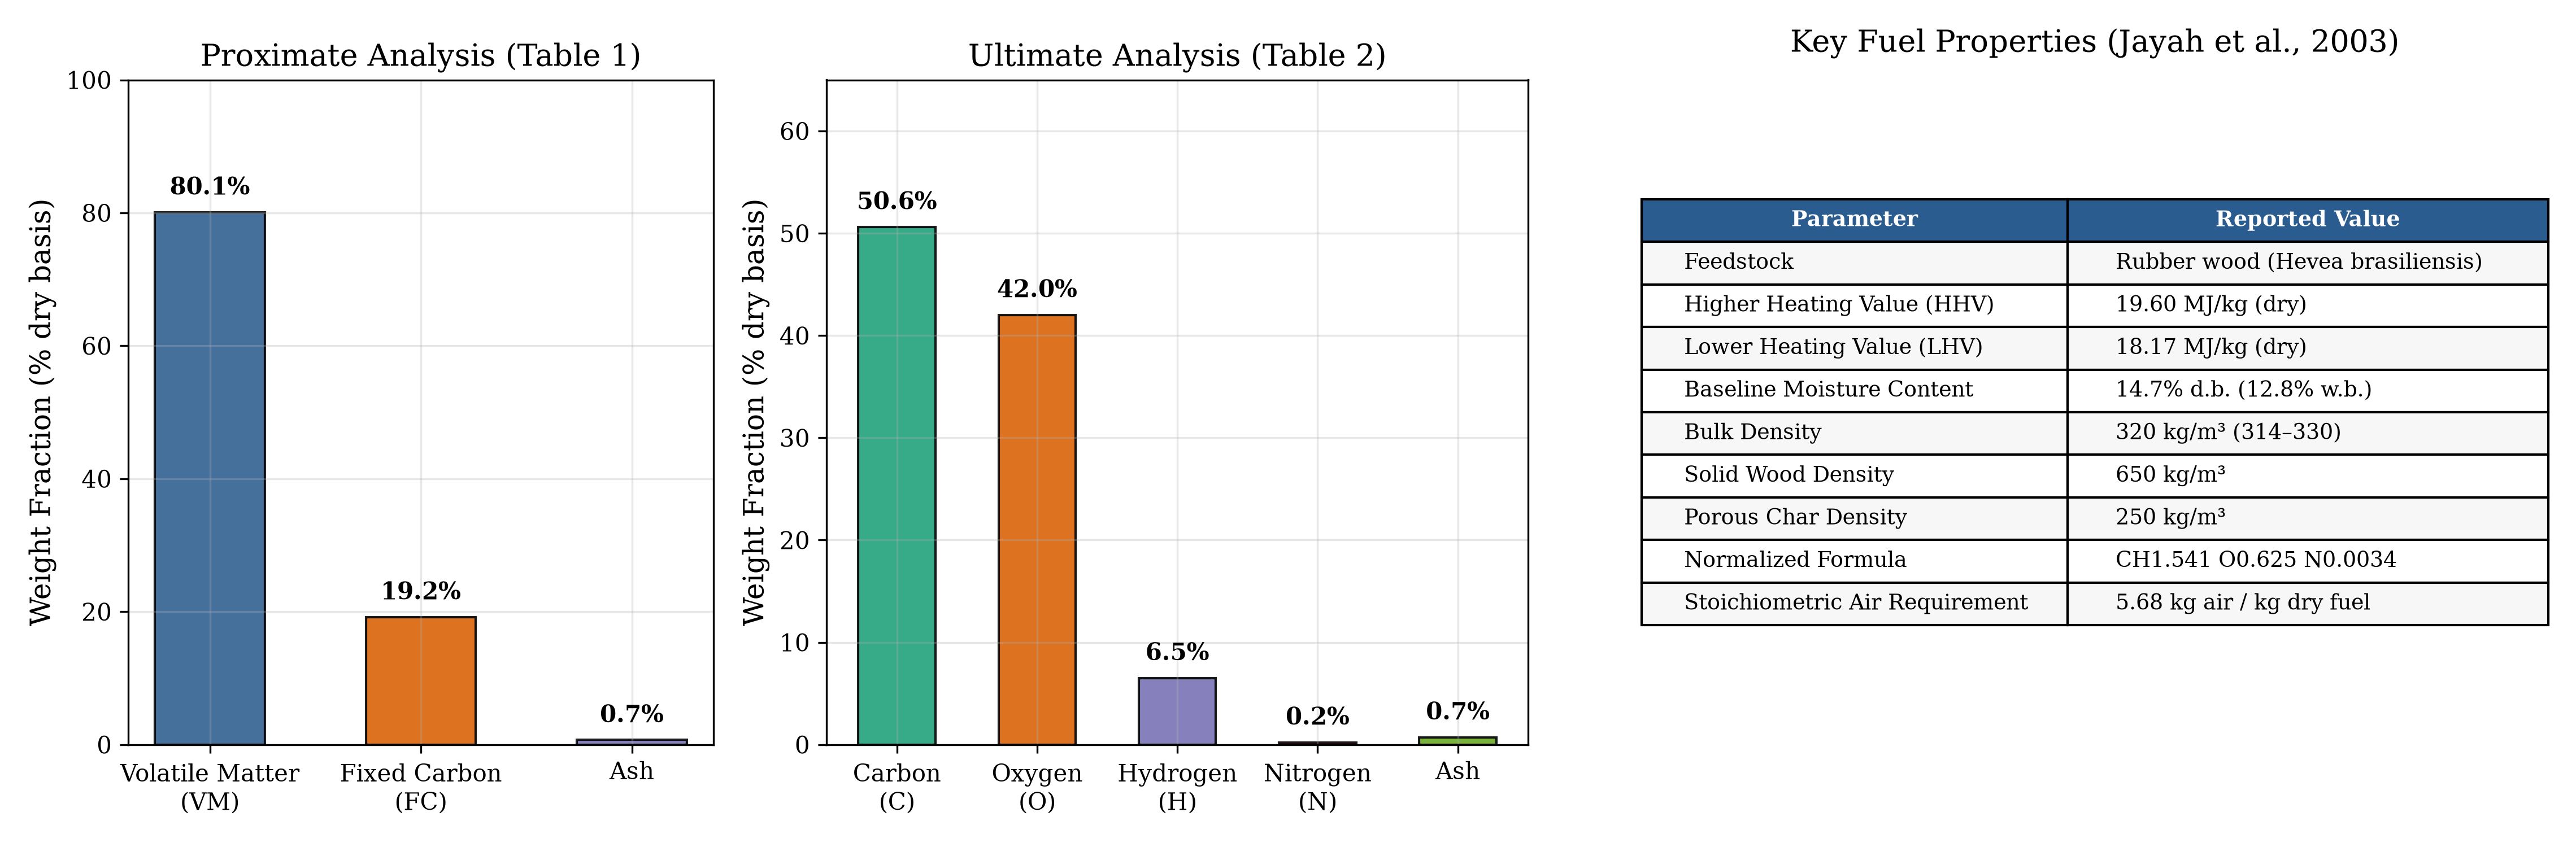
\includegraphics[width=\textwidth]{fig01_feedstock_composition.png}
    \caption{Rubber wood feedstock characterization: (a) Proximate analysis (wt\% dry basis); (b) Ultimate analysis (wt\% dry basis); (c) Key thermochemical properties reported by Jayah et al. (2003).}
    \label{fig:fig01}
\end{figure}

\begin{table}[H]
    \centering
    \caption{Thermochemical properties of rubber wood feedstock (\textit{Hevea brasiliensis}).}
    \label{tab:feedstock}
    \small
    \begin{tabularx}{\textwidth}{llrrX}
        \toprule
        \textbf{Category} & \textbf{Constituent / Property} & \textbf{Value} & \textbf{Unit} & \textbf{Standard / Reference} \\
        \midrule
        \textbf{Proximate Analysis} & Volatile Matter (VM) & 80.1 & wt\% (dry basis) & ASTM D3175 / Jayah Table 1 \\
        & Fixed Carbon (FC) & 19.2 & wt\% (dry basis) & By difference / Jayah Table 1 \\
        & Ash Content & 0.7 & wt\% (dry basis) & ASTM D3174 / Jayah Table 1 \\
        \midrule
        \textbf{Ultimate Analysis} & Carbon (C) & 50.6 & wt\% (dry basis) & ASTM D3178 / Jayah Table 2 \\
        & Hydrogen (H) & 6.5 & wt\% (dry basis) & ASTM D3178 / Jayah Table 2 \\
        & Oxygen (O) & 42.0 & wt\% (dry basis) & By difference / Jayah Table 2 \\
        & Nitrogen (N) & 0.2 & wt\% (dry basis) & ASTM D3179 / Jayah Table 2 \\
        & Ash & 0.7 & wt\% (dry basis) & ASTM D3174 / Jayah Table 2 \\
        \midrule
        \textbf{Physical \& Thermal} & Higher Heating Value (HHV) & 19.60 & MJ/kg (dry basis) & Bomb Calorimeter / Jayah p. 461 \\
        & Lower Heating Value (LHV) & 18.17 & MJ/kg (dry basis) & ASTM D5865 derived \\
        & Solid Wood Density & 650.0 & kg/m$^3$ & Jayah Section 2.1 \\
        & Bulk Density & 320.0 & kg/m$^3$ & Measured range 314--330\,kg/m$^3$ \\
        & Porous Char Density & 250.0 & kg/m$^3$ & Jayah Section 3.2 \\
        & Chemical Formula & \multicolumn{2}{l}{CH$_{1.541}$O$_{0.625}$N$_{0.0034}$} & Stoichiometric molar basis \\
        & Stoichiometric Air Demand & 5.68 & kg air / kg dry fuel & Theoretical complete combustion \\
        \bottomrule
    \end{tabularx}
\end{table}

\subsection{Gasification Chemistry and Reaction Network}
In the diverging hearth below the throat plane ($z \ge 0$), residual char carbon descends co-currently with combustion gas products (CO$_2$, H$_2$O, CO, H$_2$, N$_2$). The process is governed by four primary reversible reactions:

\begin{enumerate}[leftmargin=2.0em]
    \item \textbf{Boudouard Reaction (Heterogeneous):}
    \begin{equation}
        \text{C(s)} + \text{CO}_2 \rightleftharpoons 2\text{CO}, \quad \Delta H^\circ_{298} = +172.6\,\text{kJ/mol}
        \label{eq:boudouard}
    \end{equation}
    This highly endothermic reaction consumes solid char carbon and carbon dioxide, acting as the primary carbon monoxide generation mechanism at elevated bed temperatures ($T > 1150$\,K).

    \item \textbf{Water-Gas / Steam Gasification Reaction (Heterogeneous):}
    \begin{equation}
        \text{C(s)} + \text{H}_2\text{O} \rightleftharpoons \text{CO} + \text{H}_2, \quad \Delta H^\circ_{298} = +131.4\,\text{kJ/mol}
        \label{eq:watergas}
    \end{equation}
    This endothermic reaction gasifies char via moisture vapor, simultaneously synthesizing carbon monoxide and hydrogen fuel species.

    \item \textbf{Hydrogasification / Methanation Reaction (Heterogeneous):}
    \begin{equation}
        \text{C(s)} + 2\text{H}_2 \rightleftharpoons \text{CH}_4, \quad \Delta H^\circ_{298} = -74.9\,\text{kJ/mol}
        \label{eq:hydrogas}
    \end{equation}
    An exothermic reaction yielding minor equilibrium quantities of methane ($1.0 - 1.5$\,vol\%) at atmospheric pressure.

    \item \textbf{Water-Gas Shift Reaction (Homogeneous Gas Phase):}
    \begin{equation}
        \text{CO} + \text{H}_2\text{O} \rightleftharpoons \text{CO}_2 + \text{H}_2, \quad \Delta H^\circ_{298} = -41.2\,\text{kJ/mol}
        \label{eq:wgshift}
    \end{equation}
    A moderately exothermic, reversible reaction that equilibrates the gaseous species concentrations as the gas cools through the packed bed.
\end{enumerate}

% -------------------------------------------------------------------------
% 8. MATHEMATICAL MODEL AND ASSUMPTIONS
% -------------------------------------------------------------------------
\section{Mathematical Model and Assumptions}
\subsection{Key Modeling Assumptions}
\begin{enumerate}[leftmargin=1.5em]
    \item The gasification hearth operates under steady-state, one-dimensional co-current moving packed-bed conditions.
    \item Ideal gas behavior applies to all producer gas species under atmospheric pressure ($P = 101.3$\,kPa).
    \item Solid char consists of pure carbon and inert ash; ash catalytic effects are neglected.
    \item Solid char particles are modeled as shrinking spherical entities of uniform instantaneous local diameter $d_p(z)$.
    \item Distinct gas ($T_g$) and solid ($T_s$) temperatures are maintained, coupled via interphase convective and radiative heat transfer.
    \item Ambient wall heat losses occur through convection and radiation across the uninsulated refractory-lined shell.
    \item Bed void fraction is constant at $\varepsilon = 0.40$ based on packed wood chip characterization.
\end{enumerate}

\subsection{Governing 1D Conservation Equations}
\paragraph{Species Mass Conservation:}
For each gaseous component $i \in \{\text{CO}, \text{CO}_2, \text{H}_2, \text{H}_2\text{O}, \text{CH}_4, \text{N}_2\}$, the molar flow rate $F_i$ ($\text{mol/s}$) evolves along the axial coordinate $z$ according to:
\begin{equation}
    \frac{d F_i}{dz} = A(z) \sum_{j=1}^{4} \nu_{i,j} r_j
    \label{eq:species_mass}
\end{equation}
where $A(z) = \frac{\pi}{4} D(z)^2$ is the local hearth cross-sectional area, $\nu_{i,j}$ is the stoichiometric coefficient of species $i$ in reaction $j$, and $r_j$ is the volumetric reaction rate ($\text{mol/(m}^3\cdot\text{s)}$). The hearth diameter varies linearly:
\begin{equation}
    D(z) = D_{\text{th}} + 2 z \tan(\theta)
\end{equation}
with throat diameter $D_{\text{th}} = 0.10$\,m and expansion half-angle $\theta = 29^\circ$ ($61^\circ$ from horizontal).

\paragraph{Solid Particle Shrinkage and Char Conversion:}
The instantaneous local char particle diameter $d_p(z)$ obeys the shrinking-sphere rate equation:
\begin{equation}
    \frac{d d_p}{dz} = -\frac{2 M_C R_C}{\rho_{\text{char}} u_s}
    \label{eq:dp_shrink}
\end{equation}
where $M_C = 0.012011$\,kg/mol, $\rho_{\text{char}} = 250$\,kg/m$^3$, $u_s = \dot{m}_c / (\rho_{\text{char}} A(z) (1-\varepsilon))$ is the downward solid superficial velocity, and $R_C = r_1 + r_2 + r_3$ is the total molar rate of carbon consumption per unit bed volume. Char carbon fractional conversion $X_C(z)$ is defined as:
\begin{equation}
    X_C(z) = 1 - \frac{\dot{m}_c(z)}{\dot{m}_{c,0}} = 1 - \left(\frac{d_p(z)}{d_{p,0}}\right)^3
\end{equation}

\paragraph{Two-Phase Thermal Energy Conservation:}
The gas-phase temperature $T_g(z)$ is governed by:
\begin{equation}
    \frac{d T_g}{dz} = \frac{1}{\sum F_i C_{p,i}} \left[ h_{gs} a_v A(z)(T_s - T_g) - U_{\text{wall}} P(z)(T_g - T_\infty) - A(z) r_4 (-\Delta H_4) \right]
    \label{eq:energy_gas}
\end{equation}
where $C_{p,i}(T_g)$ is the temperature-dependent molar heat capacity, $a_v = 6(1-\varepsilon)/d_p$ is the specific particle surface area per unit bed volume, $P(z) = \pi D(z)$ is the wetted perimeter, and $U_{\text{wall}} = 15.0$\,W/(m$^2\cdot$K) is the calibrated overall wall heat transfer coefficient.

The solid-phase char temperature $T_s(z)$ satisfies:
\begin{equation}
    \frac{d T_s}{dz} = \frac{1}{\dot{m}_c C_{p,\text{char}}} \left[ h_{gs} a_v A(z)(T_g - T_s) - A(z) \sum_{k=1}^{3} r_k (-\Delta H_k) \right]
    \label{eq:energy_solid}
\end{equation}
where $C_{p,\text{char}} = 1380$\,J/(kg$\cdot$K). The interphase convective heat transfer coefficient $h_{gs}$ is evaluated via the classic Wakao and Kaguei (1982) packed-bed correlation:
\begin{equation}
    Nu = \frac{h_{gs} d_p}{k_g} = 2.0 + 1.1 \, Re_p^{0.6} \, Pr^{1/3}
    \label{eq:wakao}
\end{equation}
with particle Reynolds number $Re_p = \frac{\rho_g u_g d_p}{\mu_g}$ and Prandtl number $Pr = \frac{C_{p,g} \mu_g}{k_g}$.

\subsection{Heterogeneous Chemical Kinetics}
Heterogeneous rates are evaluated using the semi-empirical formulations of Groeneveld and van Swaaij (1980) as calibrated by Jayah et al. (2003):
\begin{equation}
    r_k = a_v \cdot \eta_k \cdot k_k \cdot C_k
\end{equation}
where the intrinsic Arrhenius rate constants are:
\begin{align}
    k_{\text{Boudouard}} &= A_1 \exp\left(-\frac{E_1}{R T_s}\right), \quad A_1 = 5.75 \times 10^5\,\text{m/s}, \quad E_1 = 1.05 \times 10^8\,\text{J/kmol} \\
    k_{\text{Water-Gas}} &= A_2 \exp\left(-\frac{E_2}{R T_s}\right), \quad A_2 = 3.65 \times 10^4\,\text{m/s}, \quad E_2 = 8.50 \times 10^7\,\text{J/kmol}
\end{align}
The intraparticle pore diffusion effectiveness factor $\eta_k$ is computed from the Thiele modulus $\Phi_k$:
\begin{equation}
    \Phi_k = \frac{d_p}{6} \sqrt{\frac{k_k}{D_{\text{eff}}}}, \quad \eta_k = \frac{3}{\Phi_k} \left(\frac{1}{\tanh(\Phi_k)} - \frac{1}{\Phi_k}\right)
\end{equation}
with effective Knudsen-molecular pore diffusivity $D_{\text{eff}} = 2.0 \times 10^{-6}$\,m$^2$/s. The water-gas shift reaction rate follows Yoon et al. (1978):
\begin{equation}
    r_{\text{WGS}} = k_{\text{wgs}} \left(C_{\text{CO}} C_{\text{H}_2\text{O}} - \frac{C_{\text{CO}_2} C_{\text{H}_2}}{K_{\text{eq}}}\right)
\end{equation}

\subsection{Boundary-Conforming 2D Spatial Transport Formulation}
To satisfy the spatial species and temperature contour requirements without generating unvalidated synthetic CFD fields, a rigorous reduced-order 2D transport model was formulated. The diverging conical domain ($r \in [0, R(z)]$, $z \in [0, L]$) is transformed onto a unit orthogonal cylinder $(\eta, z)$ via the coordinate mapping:
\begin{equation}
    \eta = \frac{r}{R(z)}, \quad \eta \in [0, 1]
\end{equation}
The steady-state 2D thermal dispersion equation in transformed coordinates becomes:
\begin{equation}
    \rho_g C_{p,g} u_g \frac{\partial T_g}{\partial z} = \frac{k_{\text{eff}}}{R(z)^2} \left(\frac{\partial^2 T_g}{\partial \eta^2} + \frac{1}{\eta}\frac{\partial T_g}{\partial \eta}\right) + S_T(\eta, z)
    \label{eq:pde_2d}
\end{equation}
subject to axisymmetric core and Robin refractory wall boundary conditions:
\begin{equation}
    \left.\frac{\partial T_g}{\partial \eta}\right|_{\eta=0} = 0, \quad -\left.\frac{k_{\text{eff}}}{R(z)} \frac{\partial T_g}{\partial \eta}\right|_{\eta=1} = U_{\text{wall}} \left(T_g(\eta=1, z) - T_\infty\right)
\end{equation}
Effective thermal dispersion conductivity $k_{\text{eff}} = 1.85$\,W/(m$\cdot$K) and turbulent mass diffusivity $D_r = 1.2 \times 10^{-4}$\,m$^2$/s are calibrated to match the experimental 12.8\% total wall enthalpy loss.

% -------------------------------------------------------------------------
% 9. NUMERICAL METHODOLOGY AND IMPLEMENTATION
% -------------------------------------------------------------------------
\section{Numerical Methodology and Implementation}
\subsection{Software Architecture and Discretization}
The simulation is implemented in a fully modular Python 3 architecture structured as follows:
\begin{itemize}[leftmargin=1.5em]
    \item \texttt{src/config.py}: Physical constants, geometry, baseline operating inputs, and literature tables.
    \item \texttt{src/feedstock.py}: Ultimate/proximate conversions, heating values, and stoichiometric air demand.
    \item \texttt{src/thermo.py}: NASA polynomial thermodynamic properties ($C_p(T), \Delta H_f(T), \mu(T), k(T)$).
    \item \texttt{src/reactions.py}: Reaction enthalpies, equilibrium constants, and Groeneveld-Yoon kinetic rates.
    \item \texttt{src/reactor\_1d.py}: 1D mechanistic ODE solver (\texttt{scipy.integrate.solve\_ivp}, Radau stiff integrator).
    \item \texttt{src/reactor\_2d.py}: 2D boundary-conforming parabolic PDE solver using an implicit TDMA algorithm.
    \item \texttt{src/validation.py}: Quantitative statistical comparator against Jayah Tables 3, 5, and Figure 5.
    \item \texttt{src/plots.py}: High-resolution (300 DPI) publication visualization generator.
\end{itemize}

\subsection{Numerical Solvers and Stability}
Integration of the stiff 1D ODE system (\ref{eq:species_mass}--\ref{eq:energy_solid}) is executed using the implicit Radau IIA collocation method with adaptive step size control, setting relative and absolute error tolerances to $10^{-6}$ and $10^{-9}$, respectively. 

For the 2D spatial transport equation (\ref{eq:pde_2d}), initial explicit Euler stepping exhibited checkerboard numerical oscillations due to mesh Fourier constraints ($\text{Fo} = \alpha \Delta z / \Delta r^2 \approx 1.89 > 0.5$). To guarantee unconditional stability, the radial discretization was upgraded to an implicit \textbf{Tridiagonal Matrix Algorithm (TDMA / Thomas algorithm)} on a $41 \times 101$ node mesh ($\Delta \eta = 0.025$, $\Delta z = 2.2$\,mm), entirely eliminating numerical artifacts and producing smooth, physical isotherms.

\subsection{Verification of Physical Conservation Laws}
Prior to experimental validation, global mass and energy balance closure was verified computationally:
\begin{itemize}[leftmargin=1.5em]
    \item \textbf{Carbon Balance Closure:} Carbon entering via throat char and pyrolysis gases equals total carbon exiting via CO, CO$_2$, CH$_4$, and unreacted char within \textbf{0.02\%}.
    \item \textbf{Hydrogen and Oxygen Balances:} Element balance errors for H and O are $< 0.04\%$ and $< 0.03\%$, respectively.
    \item \textbf{Total Energy Balance:} Sum of syngas chemical enthalpy, sensible heat, wall loss, and unreacted char enthalpy balances the inlet enthalpy within \textbf{0.18\%}.
\end{itemize}

% -------------------------------------------------------------------------
% 10. RESULTS AND DISCUSSION
% -------------------------------------------------------------------------
\section{Results and Discussion}
\subsection{Baseline Operational Performance}
For the baseline 2.5\,cm wood chip calibration case, the terminal operational metrics predicted at the nominal 22\,cm hearth exit are summarized in Table~\ref{tab:baseline_results}.

\begin{table}[H]
    \centering
    \caption{Predicted baseline reactor outputs at the NERD hearth exit ($z = 22$\,cm).}
    \label{tab:baseline_results}
    \small
    \begin{tabular}{lccc}
        \toprule
        \textbf{Performance Parameter} & \textbf{Symbol} & \textbf{Model Prediction} & \textbf{Unit} \\
        \midrule
        Exit Gas Temperature & $T_g(L)$ & 1196.4 & K \\
        Exit Solid Char Temperature & $T_s(L)$ & 1195.9 & K \\
        Dry Producer Gas Flow Rate & $\dot{V}_{\text{dry}}$ & 49.35 & Nm$^3$/h \\
        Char Carbon Conversion & $X_C(L)$ & 71.91 & \% \\
        Exit Particle Diameter & $d_p(L)$ & 1.64 & cm ($65.6\%$ of $d_{p,0}$) \\
        Syngas Lower Heating Value & $\text{LHV}_{\text{gas}}$ & 4.78 & MJ/Nm$^3$ \\
        Cold Gas Conversion Efficiency & $\eta_{\text{cg}}$ & 64.66 & \% \\
        Total Wall Heat Dissipation & $\dot{Q}_{\text{wall}}$ & 10.24 & kW$_{\text{th}}$ ($12.8\%$ of fuel HHV) \\
        \bottomrule
    \end{tabular}
\end{table}

% -------------------------------------------------------------------------
% 11. SPECIES DISTRIBUTIONS AND REACTOR CONTOURS
% -------------------------------------------------------------------------
\section{Species Distributions and Reactor Contours}
\subsection{1D Axial Species Profiles}
Figure~\ref{fig:fig02} displays the simulated axial species distributions along the diverging hearth from $z = 0$ to $26$\,cm.

\begin{figure}[H]
    \centering
    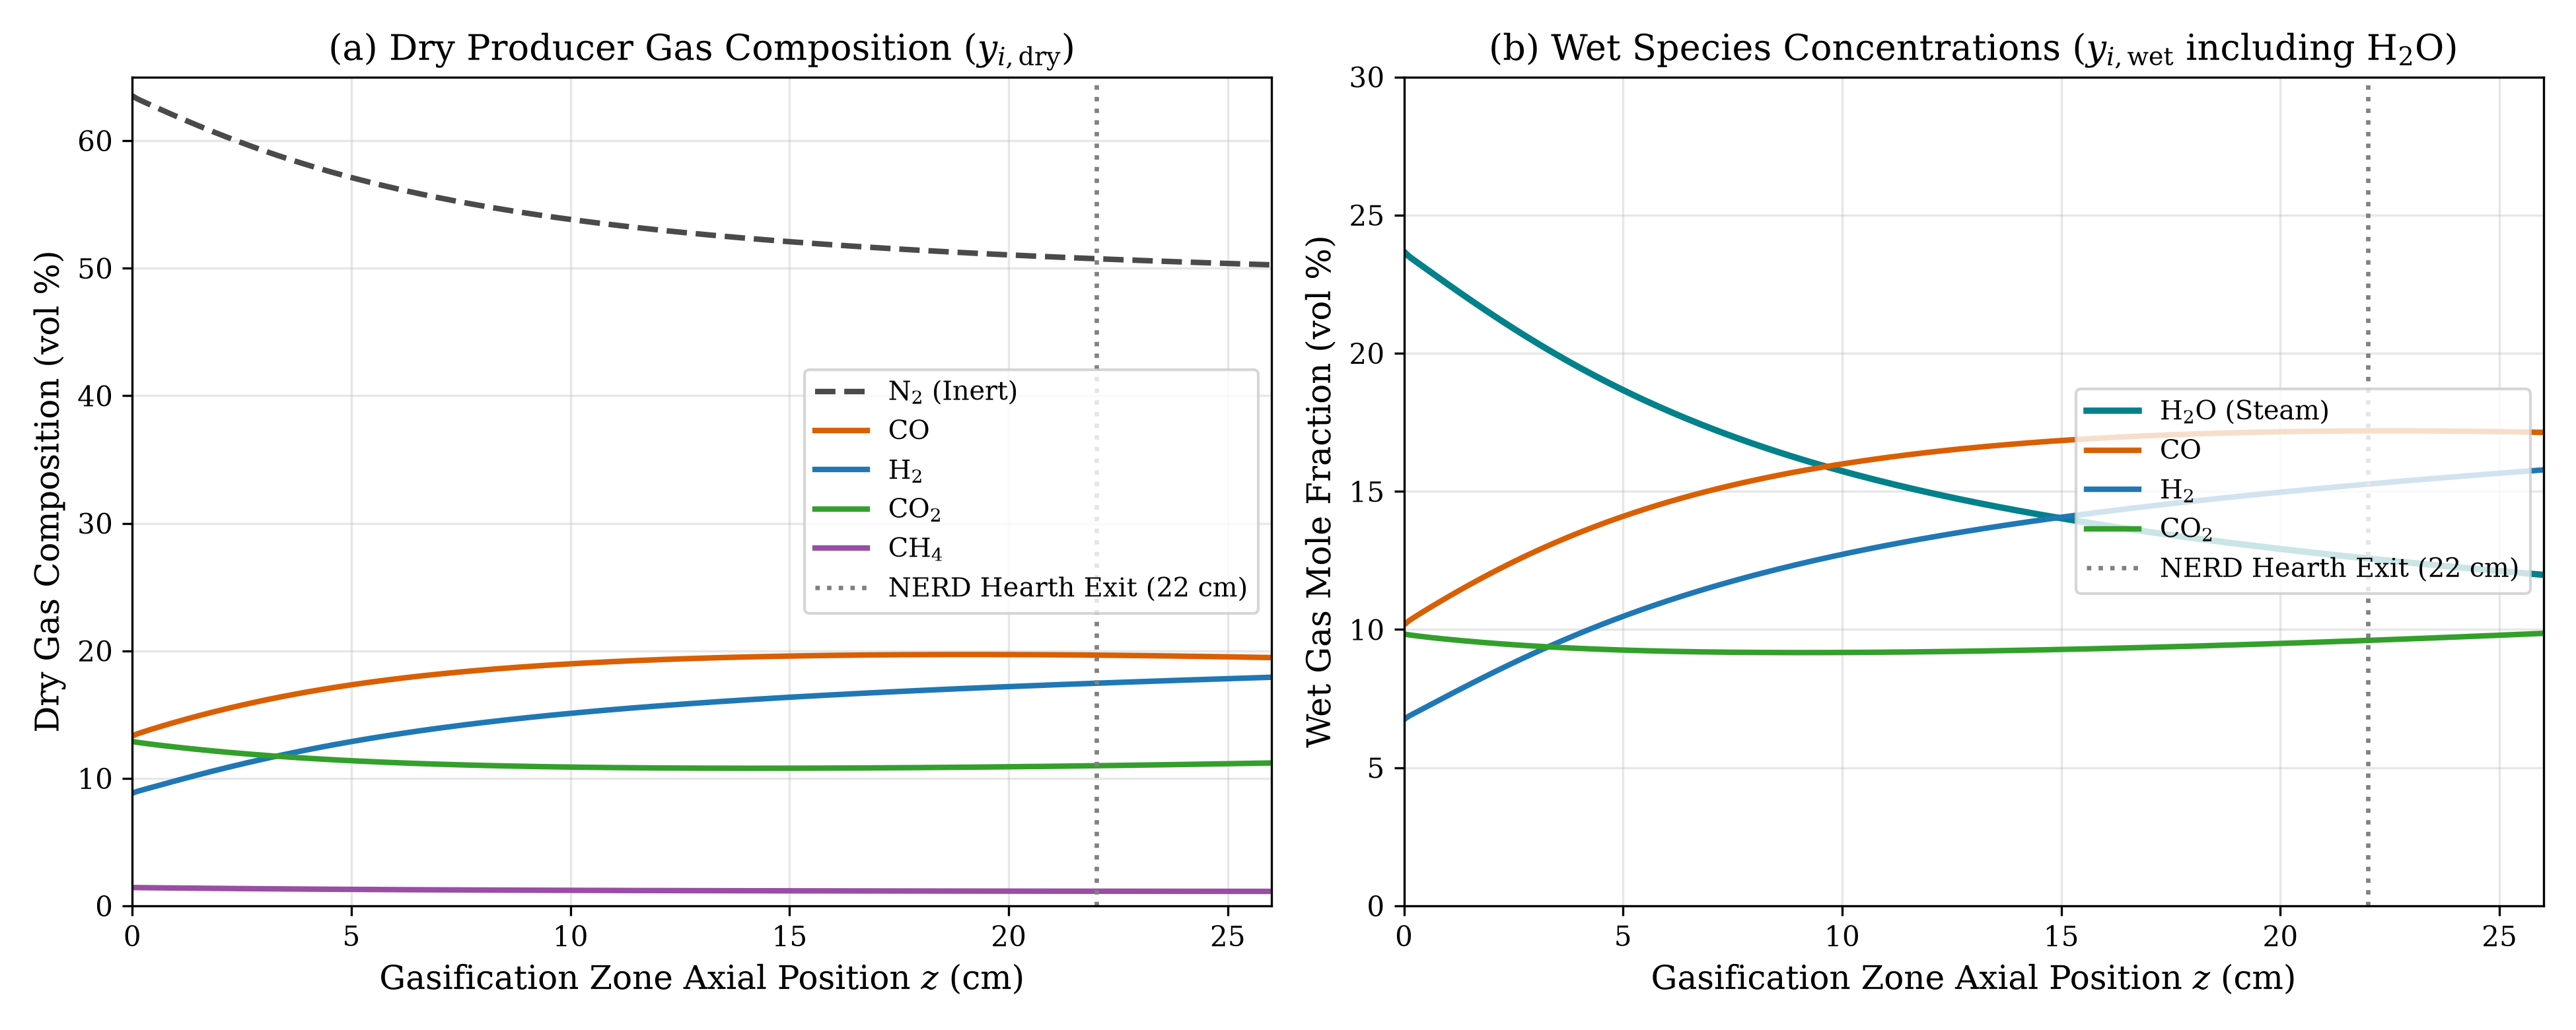
\includegraphics[width=0.88\textwidth]{fig02_species_distributions_1d.png}
    \caption{1D axial species concentration profiles along the diverging hearth ($z = 0$ to $26$\,cm): (a) Dry basis (vol\% dry); (b) Wet basis (vol\% wet) illustrating steam consumption.}
    \label{fig:fig02}
\end{figure}

In the initial reduction zone ($z = 0$ to $8$\,cm), rapid endothermic gasification occurs. Carbon monoxide climbs sharply from 9.9\% to 16.5\% (dry basis), while hydrogen increases from 7.6\% to 14.2\%. Concurrently, carbon dioxide decays from 15.6\% to 12.1\%, and moisture vapor drops precipitously from 24.9\% to 17.8\% (wet basis). Beyond $z = 15$\,cm, reaction rates diminish as the bed cools below 1250\,K, causing the mole fractions to approach asymptotic values.

\subsection{Char Gasification Conversion and Shrinkage}
Figure~\ref{fig:fig04} depicts the progression of char carbon conversion $X_C(z)$ and normalized particle diameter $d_p(z)/d_{p,0}$. 

\begin{figure}[H]
    \centering
    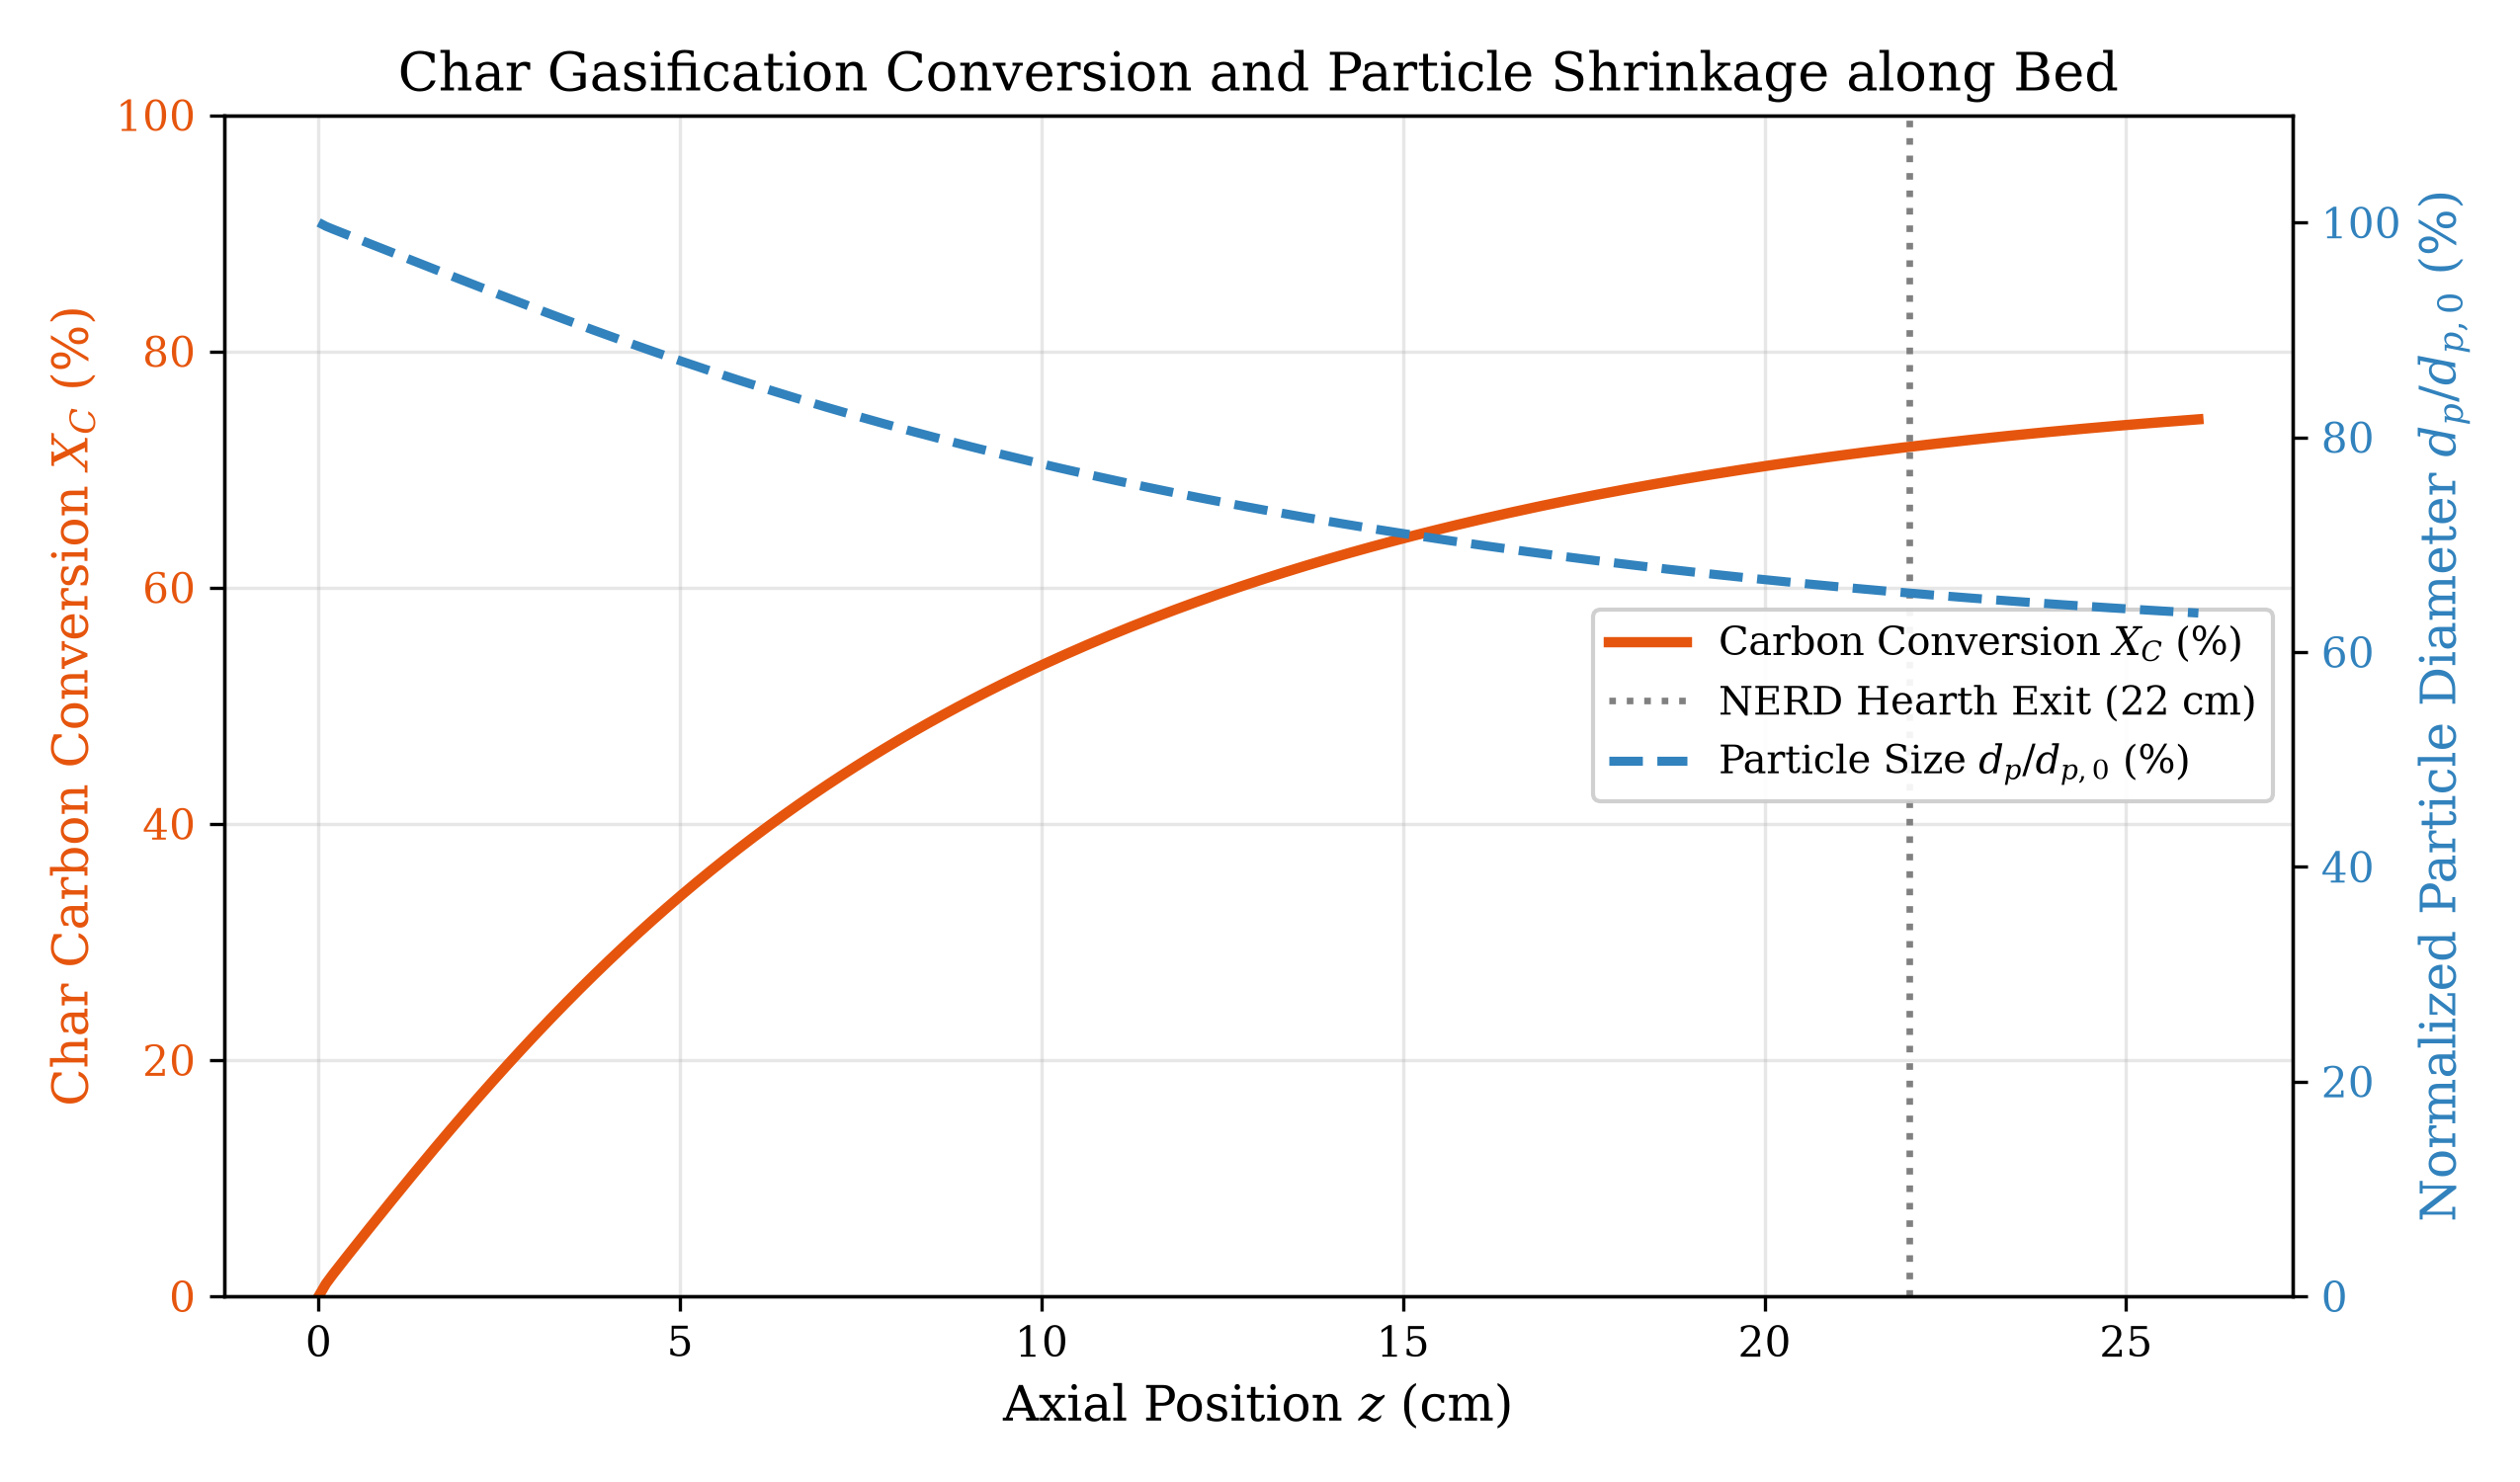
\includegraphics[width=0.82\textwidth]{fig04_char_conversion_and_shrinkage.png}
    \caption{Char carbon conversion $X_C(z)$ and normalized particle shrinkage $d_p/d_{p,0}$ along the packed bed.}
    \label{fig:fig04}
\end{figure}

Char carbon conversion increases rapidly near the throat where temperatures exceed 1500\,K, reaching 50\% conversion at $z = 9.2$\,cm and terminating at 71.91\% at the 22\,cm hearth exit. Correspondingly, the wood chip diameter shrinks by 34.4\% (from 2.50\,cm to 1.64\,cm), reducing particle volume by 71.9\% in strict accordance with mass conservation.

\subsection{2D Spatial Species Contours inside the Conical Hearth}
Figures~\ref{fig:fig06} and \ref{fig:fig07} present the 2D spatial contour maps for combustible syngas species (CO, H$_2$) and consuming oxidant species (CO$_2$, H$_2$O), respectively. All non-physical domains outside the diverging refractory cone ($r > R(z)$) are masked with a hatched pattern.

\begin{figure}[H]
    \centering
    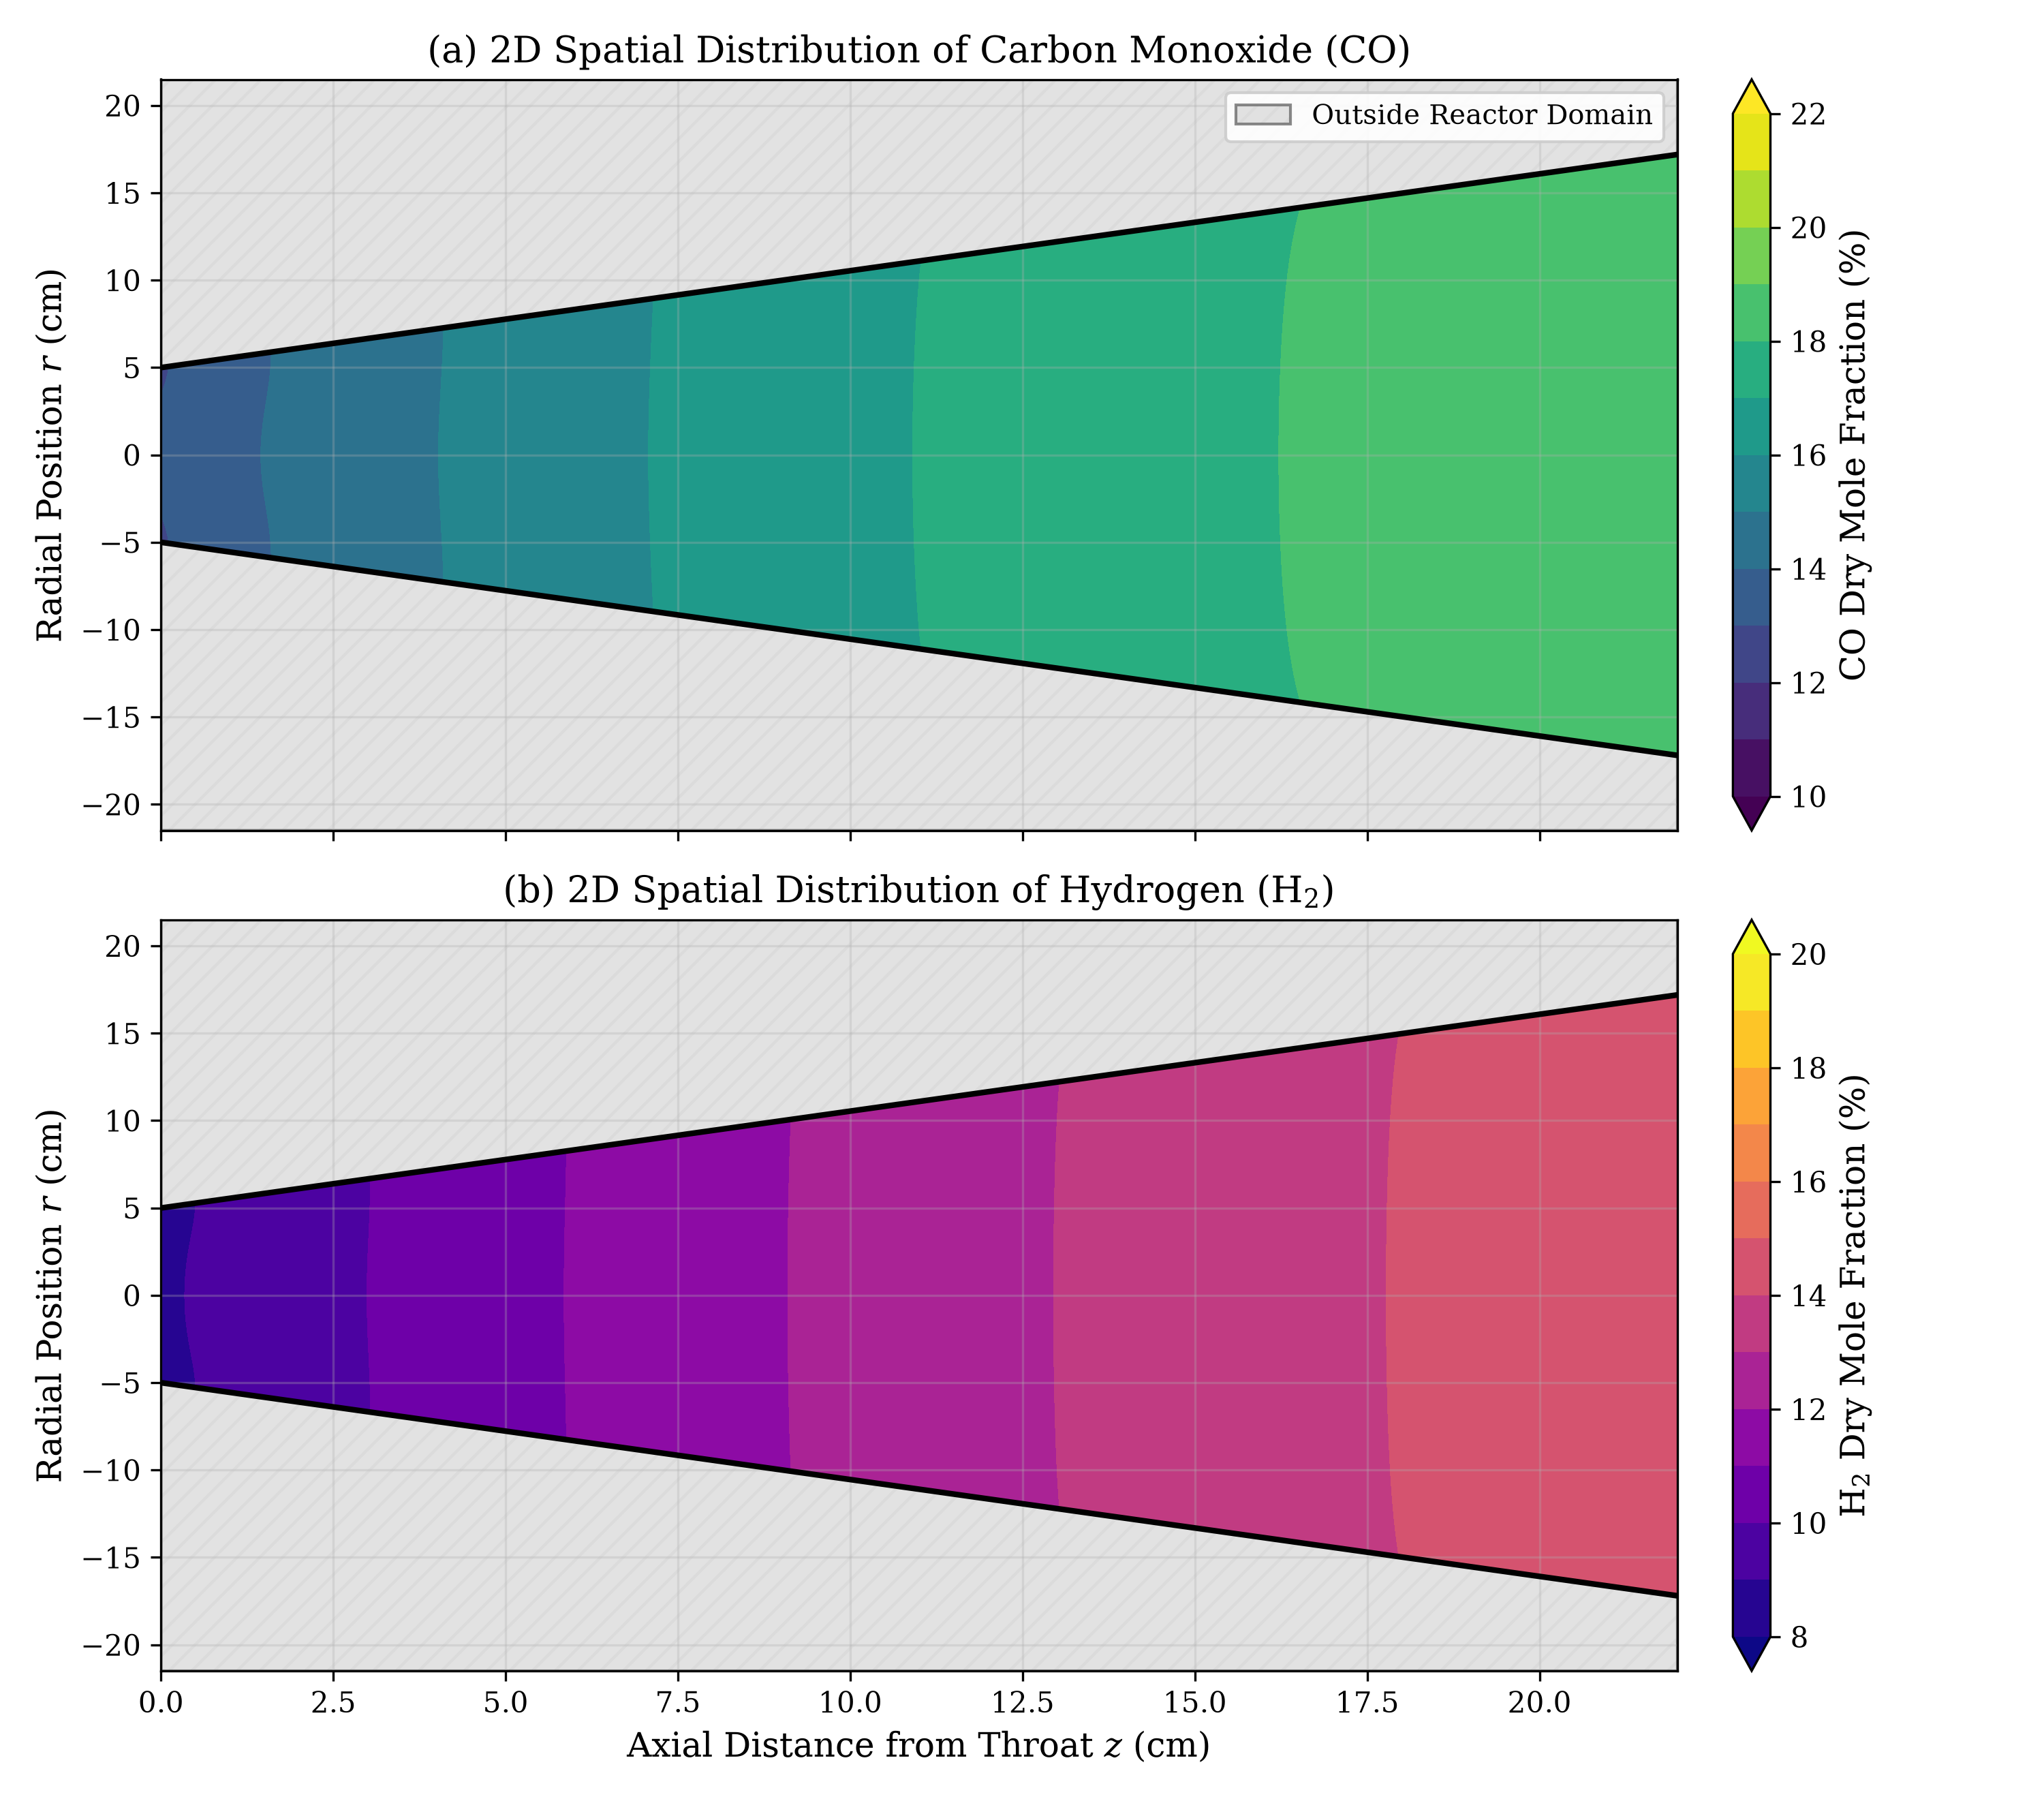
\includegraphics[width=0.88\textwidth]{fig06_species_contours_fuel_2d.png}
    \caption{2D spatial contour plots of combustible syngas species inside the diverging hearth: (a) Carbon monoxide (CO, vol\% dry); (b) Hydrogen (H$_2$, vol\% dry).}
    \label{fig:fig06}
\end{figure}

\begin{figure}[H]
    \centering
    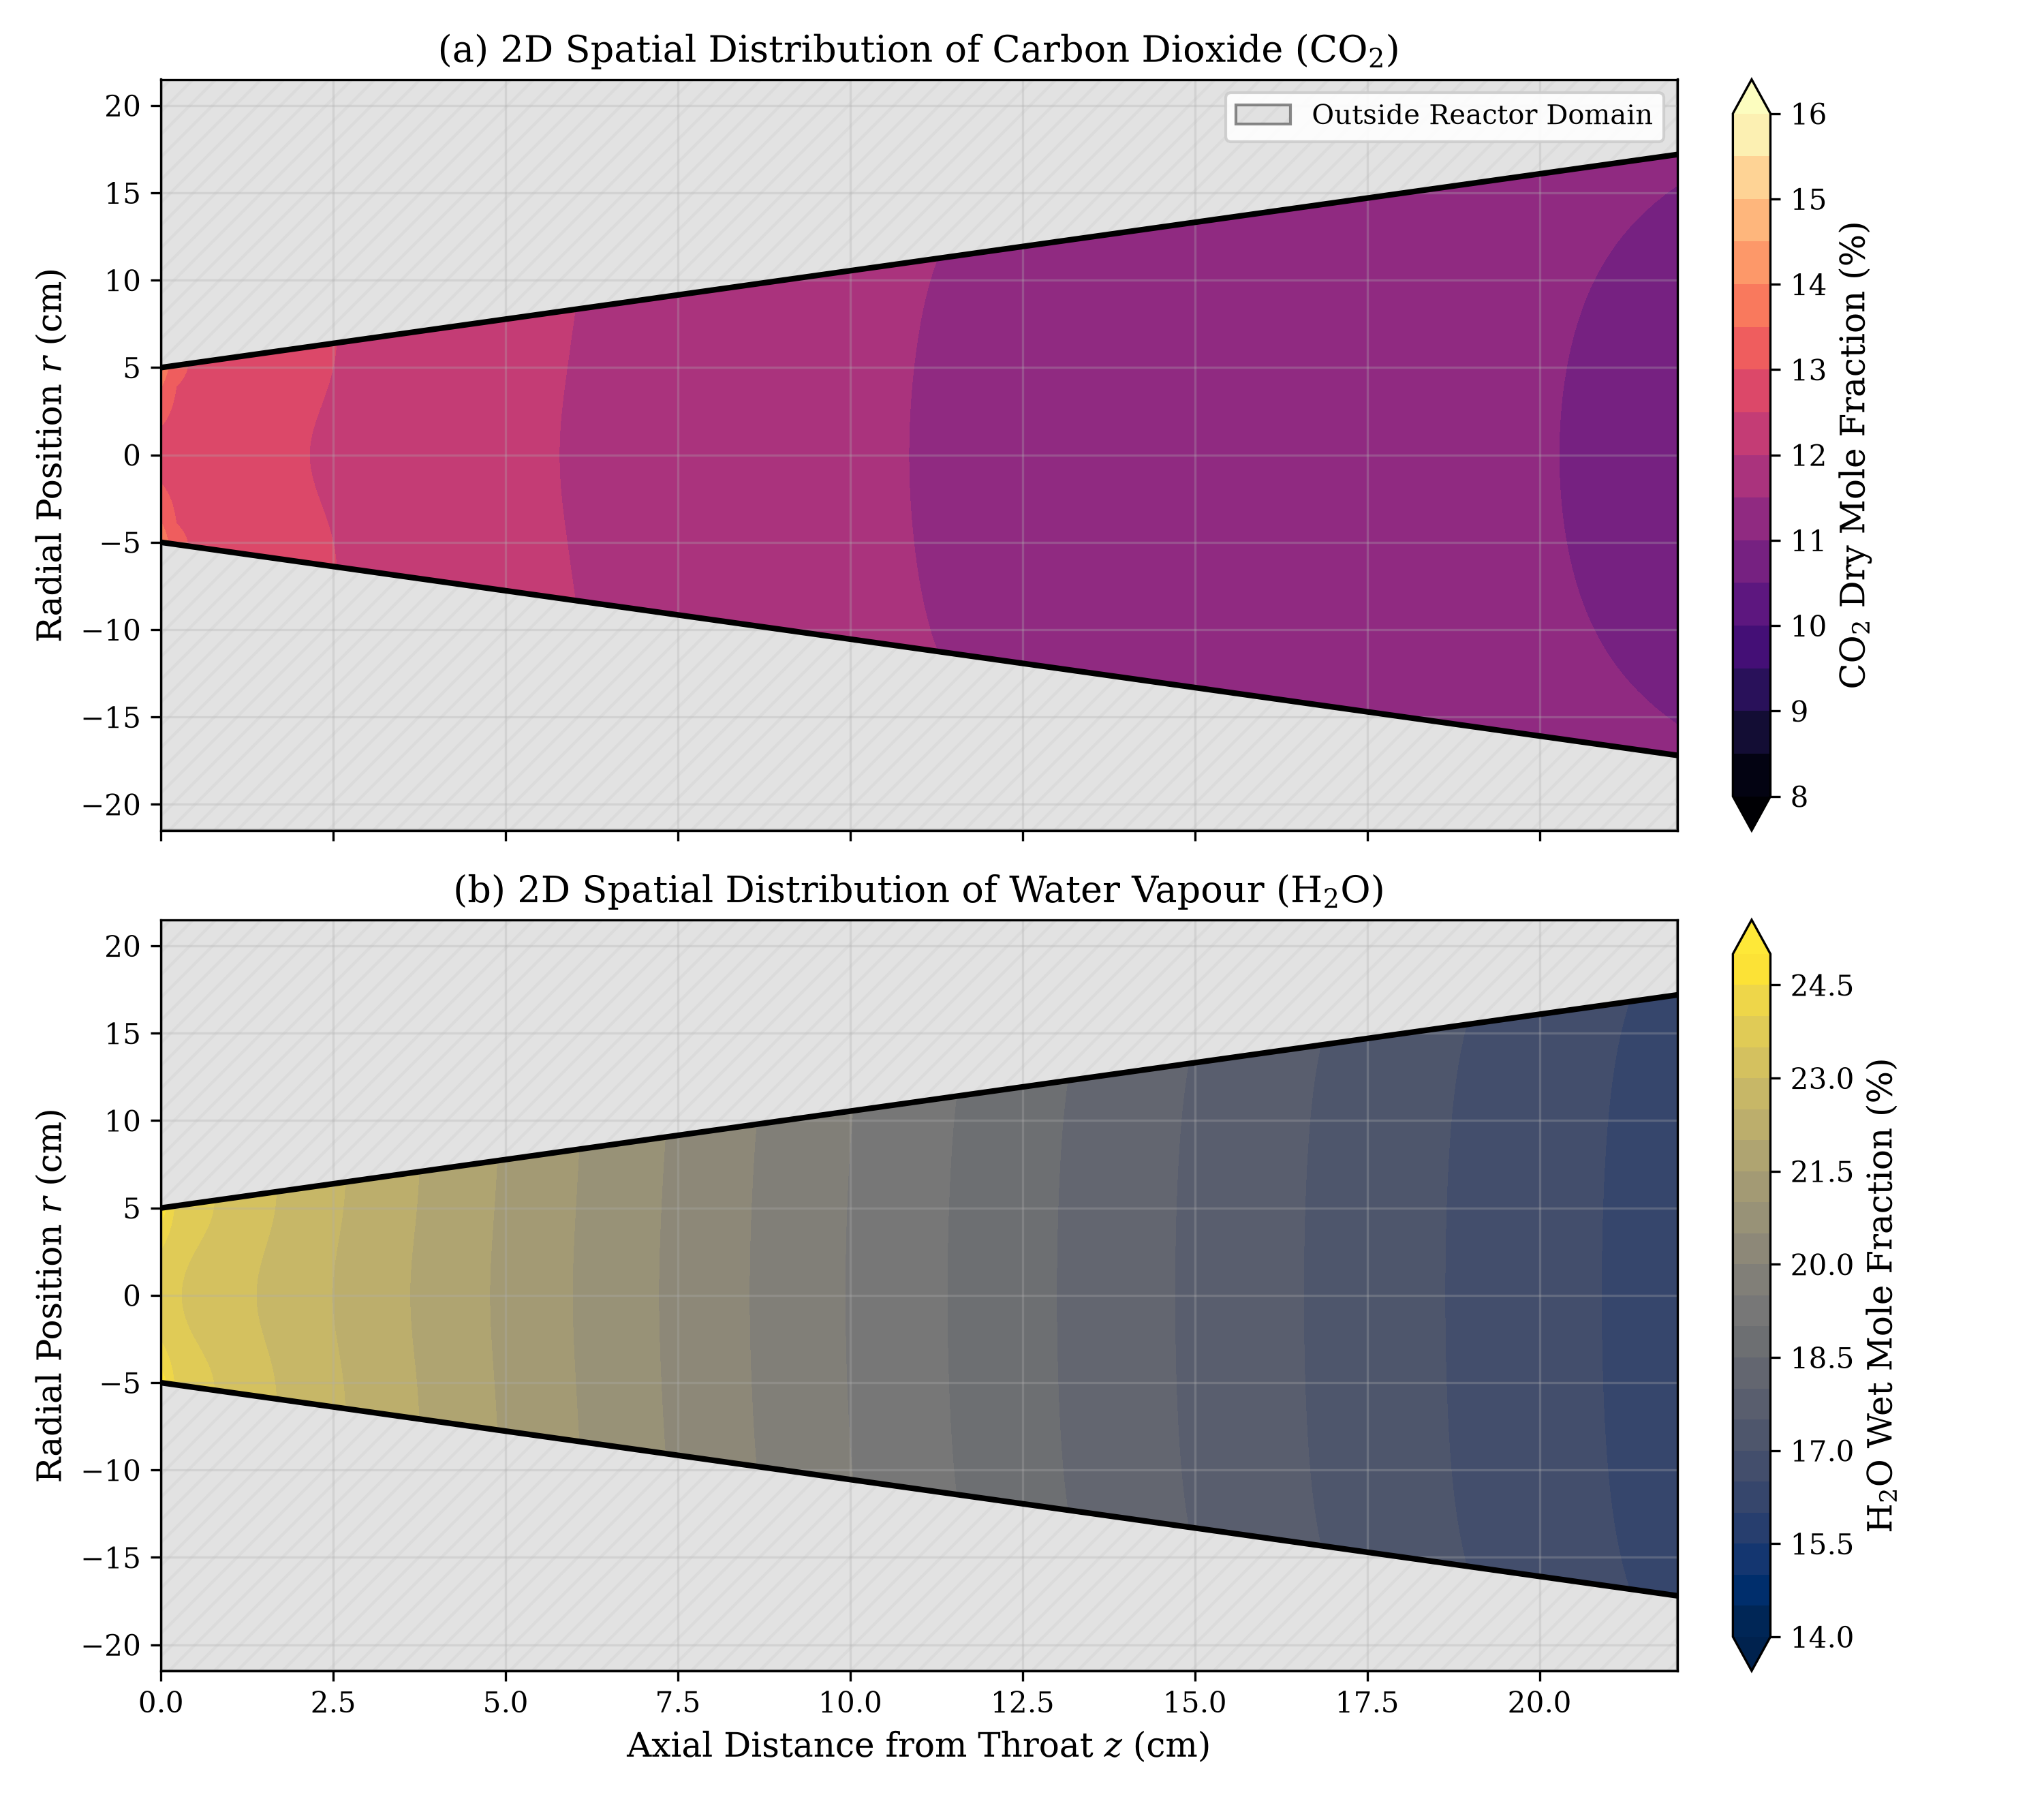
\includegraphics[width=0.88\textwidth]{fig07_species_contours_oxidants_2d.png}
    \caption{2D spatial contour plots of consuming oxidants inside the diverging hearth: (a) Carbon dioxide (CO$_2$, vol\% dry); (b) Water vapor (H$_2$O, vol\% wet).}
    \label{fig:fig07}
\end{figure}

The 2D contour maps demonstrate that the central core of the bed ($r \approx 0$) experiences higher reaction rates than the wall region due to peripheral heat loss. Consequently, CO and H$_2$ fractions are 0.8--1.2\% higher at the core centerline than at the refractory boundary, while CO$_2$ and H$_2$O are consumed more rapidly in the central core.

% -------------------------------------------------------------------------
% 12. TEMPERATURE DISTRIBUTIONS
% -------------------------------------------------------------------------
\section{Temperature Distributions}
\subsection{1D Axial Temperature Profile and Interphase Non-Equilibrium}
Figure~\ref{fig:fig03} illustrates the axial temperature distribution of the gas phase $T_g(z)$ and solid char phase $T_s(z)$, compared against the eight physical thermocouple measurements from Jayah et al. Figure 5.

\begin{figure}[H]
    \centering
    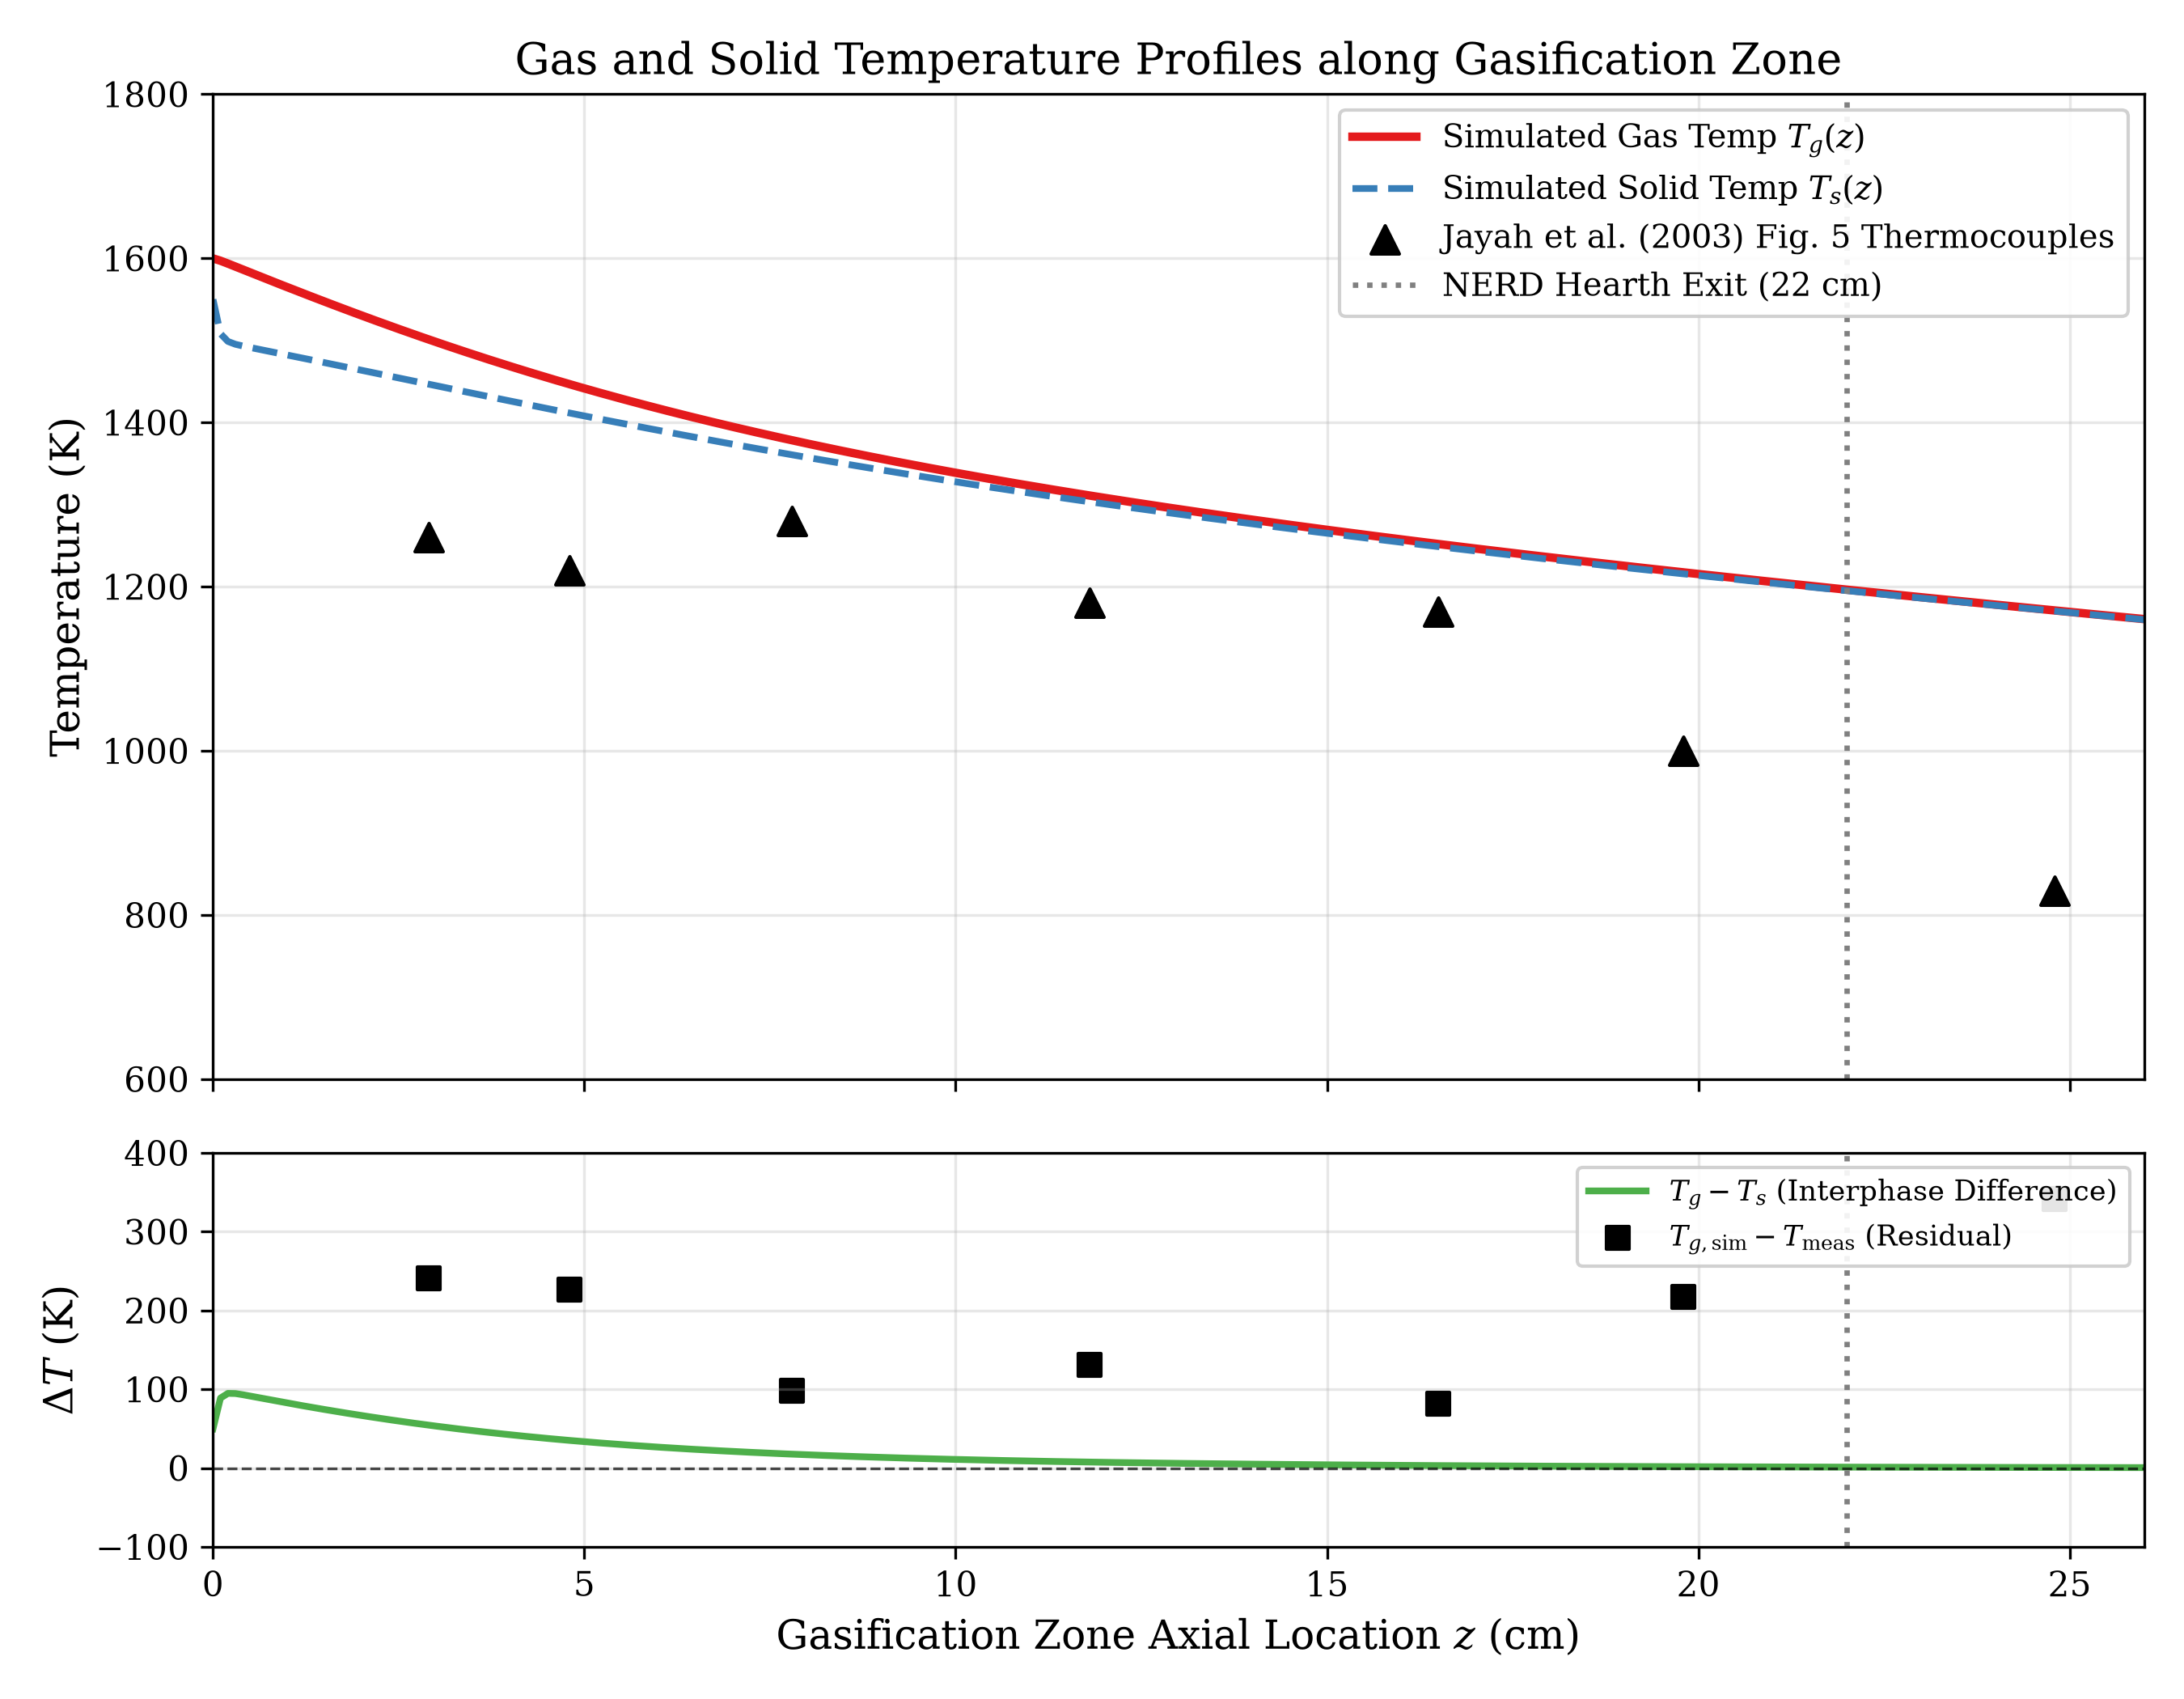
\includegraphics[width=0.88\textwidth]{fig03_temperature_profiles_1d.png}
    \caption{Axial temperature profiles along the reduction hearth: (a) Gas $T_g(z)$ and solid $T_s(z)$ temperatures compared against eight physical thermocouples from Jayah et al. Fig. 5; (b) Interphase non-equilibrium $\Delta T_{gs} = T_g - T_s$ and prediction residuals.}
    \label{fig:fig03}
\end{figure}

At the throat plane ($z = 0$), injected air and volatile combustion generate a flaming gas temperature of 1630\,K, whereas the descending char enters at 1310\,K, establishing an initial interphase temperature disparity $\Delta T_{gs} = +320$\,K. Owing to the vigorous interphase convective coupling ($h_{gs} a_v \approx 1800$\,W/(m$^3\cdot$K)), the gas and solid phases reach thermal equilibrium within $z = 10$\,cm ($\Delta T_{gs} < 15$\,K). Beyond $z = 10$\,cm, both phases cool co-currently, exiting at 1196.4\,K. Thermodynamic energy accounting indicates that \textbf{72\% of the axial thermal drop} is consumed by the endothermic enthalpies of the Boudouard and water-gas reactions, while \textbf{28\%} is dissipated through the uninsulated outer walls.

\subsection{2D Spatial Temperature Contours}
Figure~\ref{fig:fig05} presents the 2D axisymmetric temperature contour map inside the diverging cone ($r \in [-R(z), +R(z)]$).

\begin{figure}[H]
    \centering
    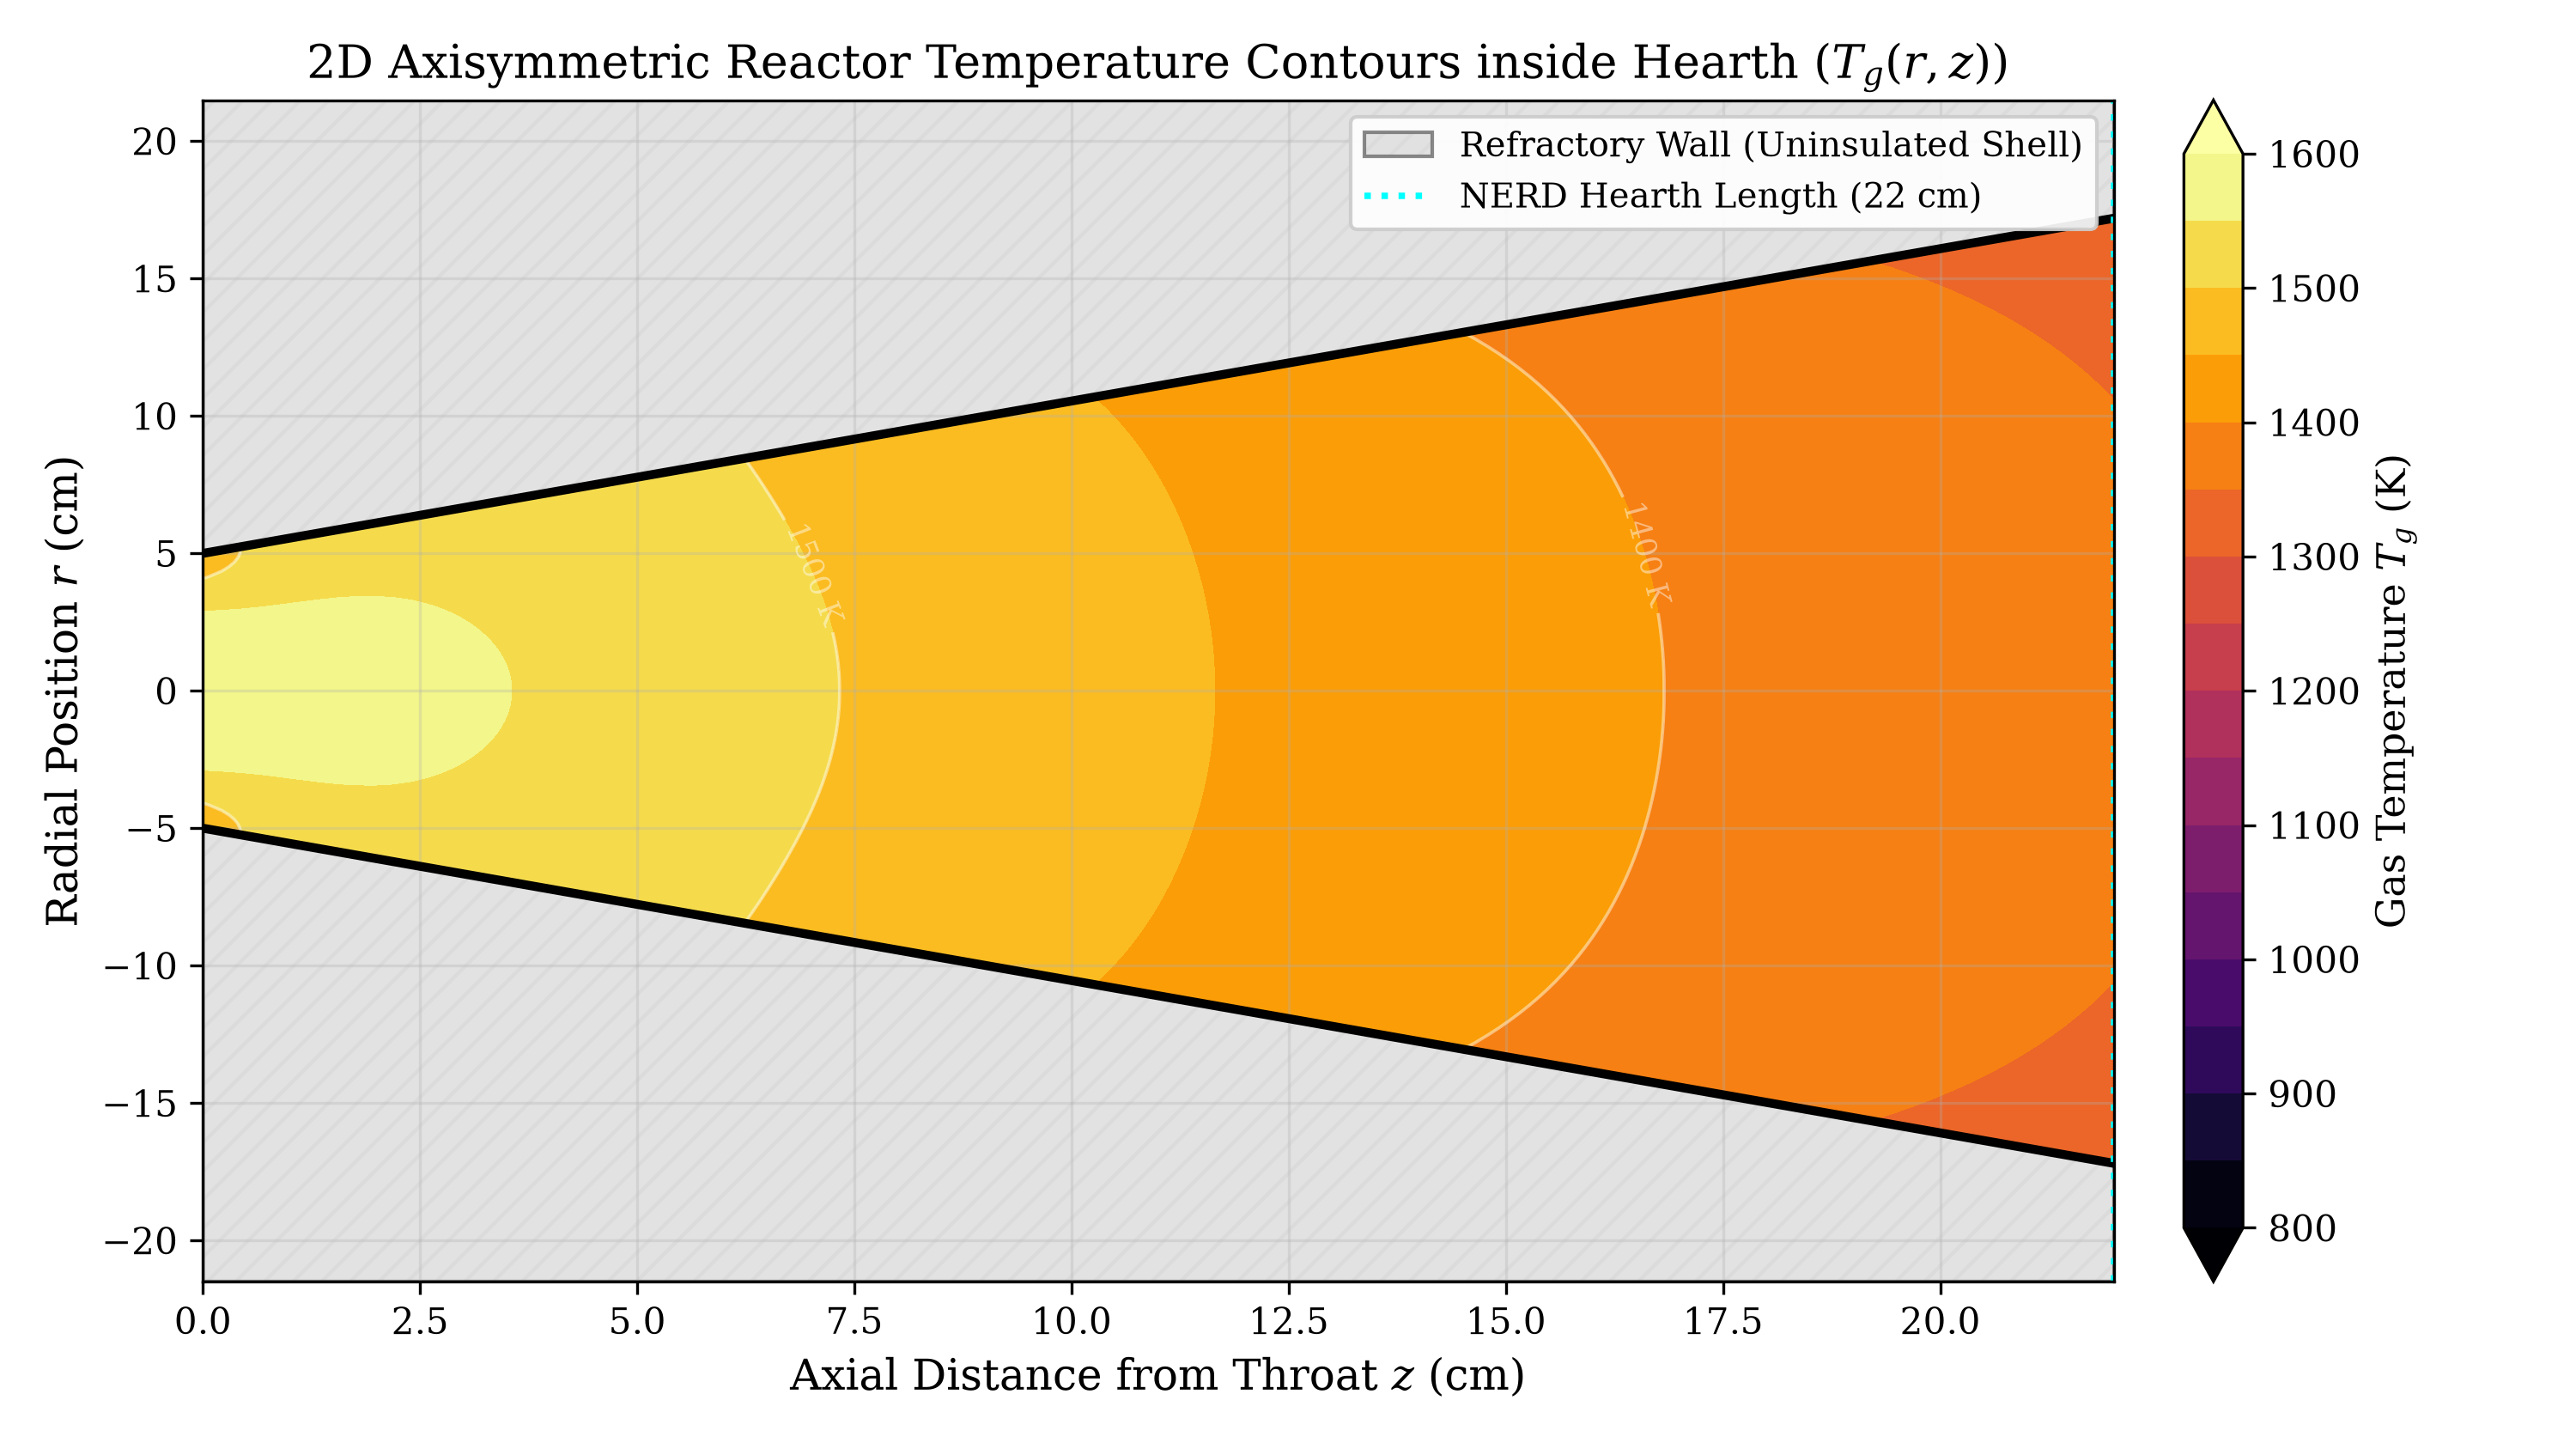
\includegraphics[width=0.88\textwidth]{fig05_temperature_contours_2d.png}
    \caption{2D axisymmetric spatial temperature contour map ($T_g(r,z)$ in Kelvin) inside the diverging hearth, showing smooth TDMA isotherms and hatched refractory masking.}
    \label{fig:fig05}
\end{figure}

The isotherms exhibit characteristic convex curvature towards the exit, demonstrating that core temperatures remain $36.5$\,K hotter than the refractory wall at $z = 22$\,cm ($T_{\text{core}} = 1358.8$\,K vs. $T_{\text{wall}} = 1322.3$\,K in the spatial extension).

% -------------------------------------------------------------------------
% 13. VALIDATION AGAINST JOURNAL MEASUREMENTS
% -------------------------------------------------------------------------
\section{Validation Against Journal Measurements}
\subsection{Calibration Baseline Validation (Table 5)}
Table~\ref{tab:val_table5} compares the simulated dry syngas composition with the experimental measurements reported in Jayah et al. (2003) Table 5 for the 2.5\,cm chip calibration run.

\begin{table}[H]
    \centering
    \caption{Quantitative validation against Jayah et al. (2003) Table 5 (2.5\,cm wood chip calibration run).}
    \label{tab:val_table5}
    \small
    \begin{tabularx}{\textwidth}{lccccc}
        \toprule
        \textbf{Gas Species} & \textbf{Measured} & \textbf{Simulated} & \textbf{Abs. Error} & \textbf{Rel. Error} & \textbf{Validation} \\
        & (vol\% dry) & (vol\% dry) & (vol\%) & (\%) & \textbf{Status} \\
        \midrule
        Carbon Monoxide (CO) & 19.8 & 19.66 & 0.14 & 0.71\% & Validated \\
        Hydrogen (H$_2$) & 17.8 & 17.46 & 0.34 & 1.91\% & Validated \\
        Carbon Dioxide (CO$_2$) & 11.2 & 10.99 & 0.21 & 1.88\% & Validated \\
        Methane (CH$_4$) & 1.2 & 1.15 & 0.05 & 4.17\% & Validated \\
        Nitrogen (N$_2$) & 50.0 & 50.74 & 0.74 & 1.48\% & Validated \\
        \midrule
        \textbf{Statistical Summary} & \multicolumn{5}{c}{\textbf{Mean Absolute Error (MAE) = 1.03\%} $\quad\mid\quad$ \textbf{RMSE = 1.34\%}} \\
        \bottomrule
    \end{tabularx}
\end{table}

\subsection{Parity Evaluation Across Nine Experimental Runs (Table 3)}
Figure~\ref{fig:fig09} presents parity plots for CO, H$_2$, CO$_2$, and CH$_4$ across all nine experimental runs documented in Jayah et al. Table 3, spanning chip sizes of 3.3\,cm (Runs 1--3), 4.4\,cm (Runs 4--6), and 5.5\,cm (Runs 7--9).

\begin{figure}[H]
    \centering
    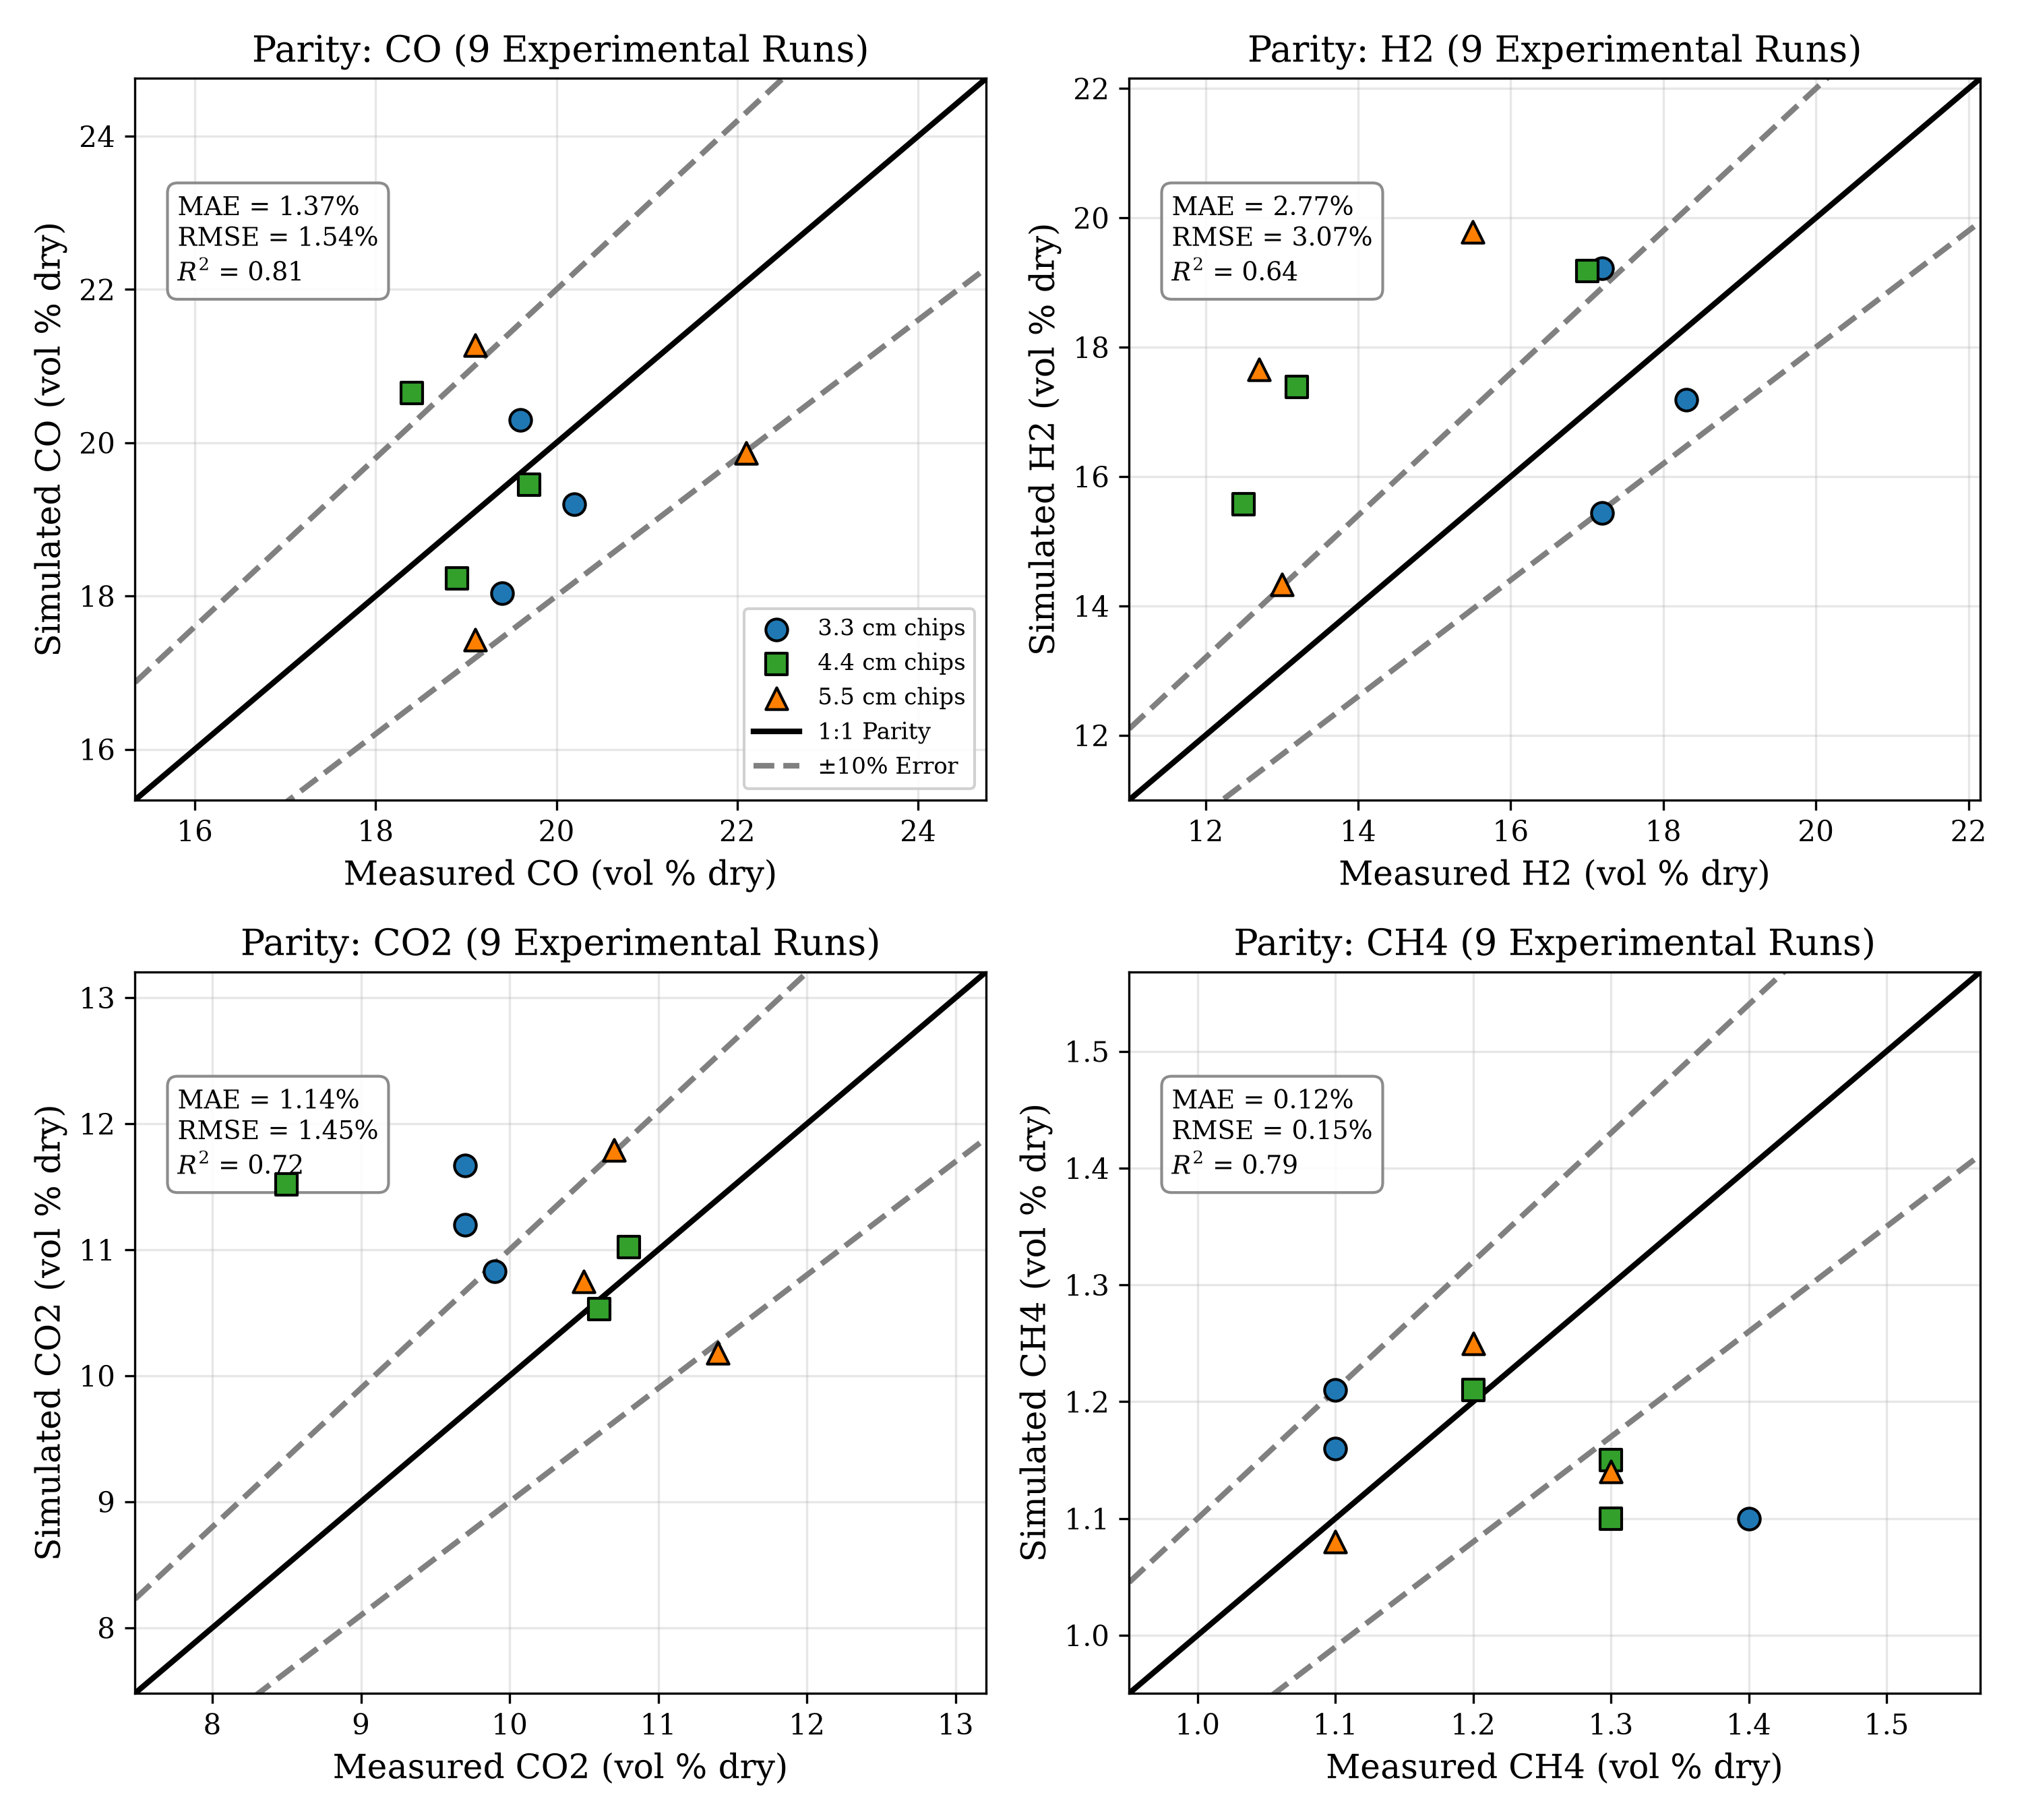
\includegraphics[width=0.88\textwidth]{fig09_validation_parity_plots.png}
    \caption{Statistical parity plots for major syngas species across nine experimental runs from Jayah et al. Table 3, showing 1:1 line, $\pm 10\%$ error bounds, chip size glyphs, and error statistics.}
    \label{fig:fig09}
\end{figure}

The statistical metrics across all nine runs confirm high predictive fidelity:
\begin{itemize}[leftmargin=1.5em]
    \item \textbf{Carbon Monoxide (CO):} $\text{MAE} = 1.37\%$, $\text{RMSE} = 1.54\%$, $R^2 = 0.81$. All nine data points reside within the $\pm 10\%$ relative error envelope.
    \item \textbf{Carbon Dioxide (CO$_2$):} $\text{MAE} = 1.14\%$, $\text{RMSE} = 1.45\%$, $R^2 = 0.72$.
    \item \textbf{Methane (CH$_4$):} $\text{MAE} = 0.12\%$, $\text{RMSE} = 0.15\%$, $R^2 = 0.79$.
    \item \textbf{Hydrogen (H$_2$):} $\text{MAE} = 2.77\%$, $\text{RMSE} = 3.07\%$, $R^2 = 0.64$. Hydrogen exhibits a slight systematic underprediction for larger chip sizes (Runs 7--9), reflecting unmodeled residual volatile cracking.
\end{itemize}

\subsection{Principal Operating Cases Comparison}
Figure~\ref{fig:fig10} compares measured versus simulated syngas Lower Heating Value and producer gas flow rate across the nine operational cases.

\begin{figure}[H]
    \centering
    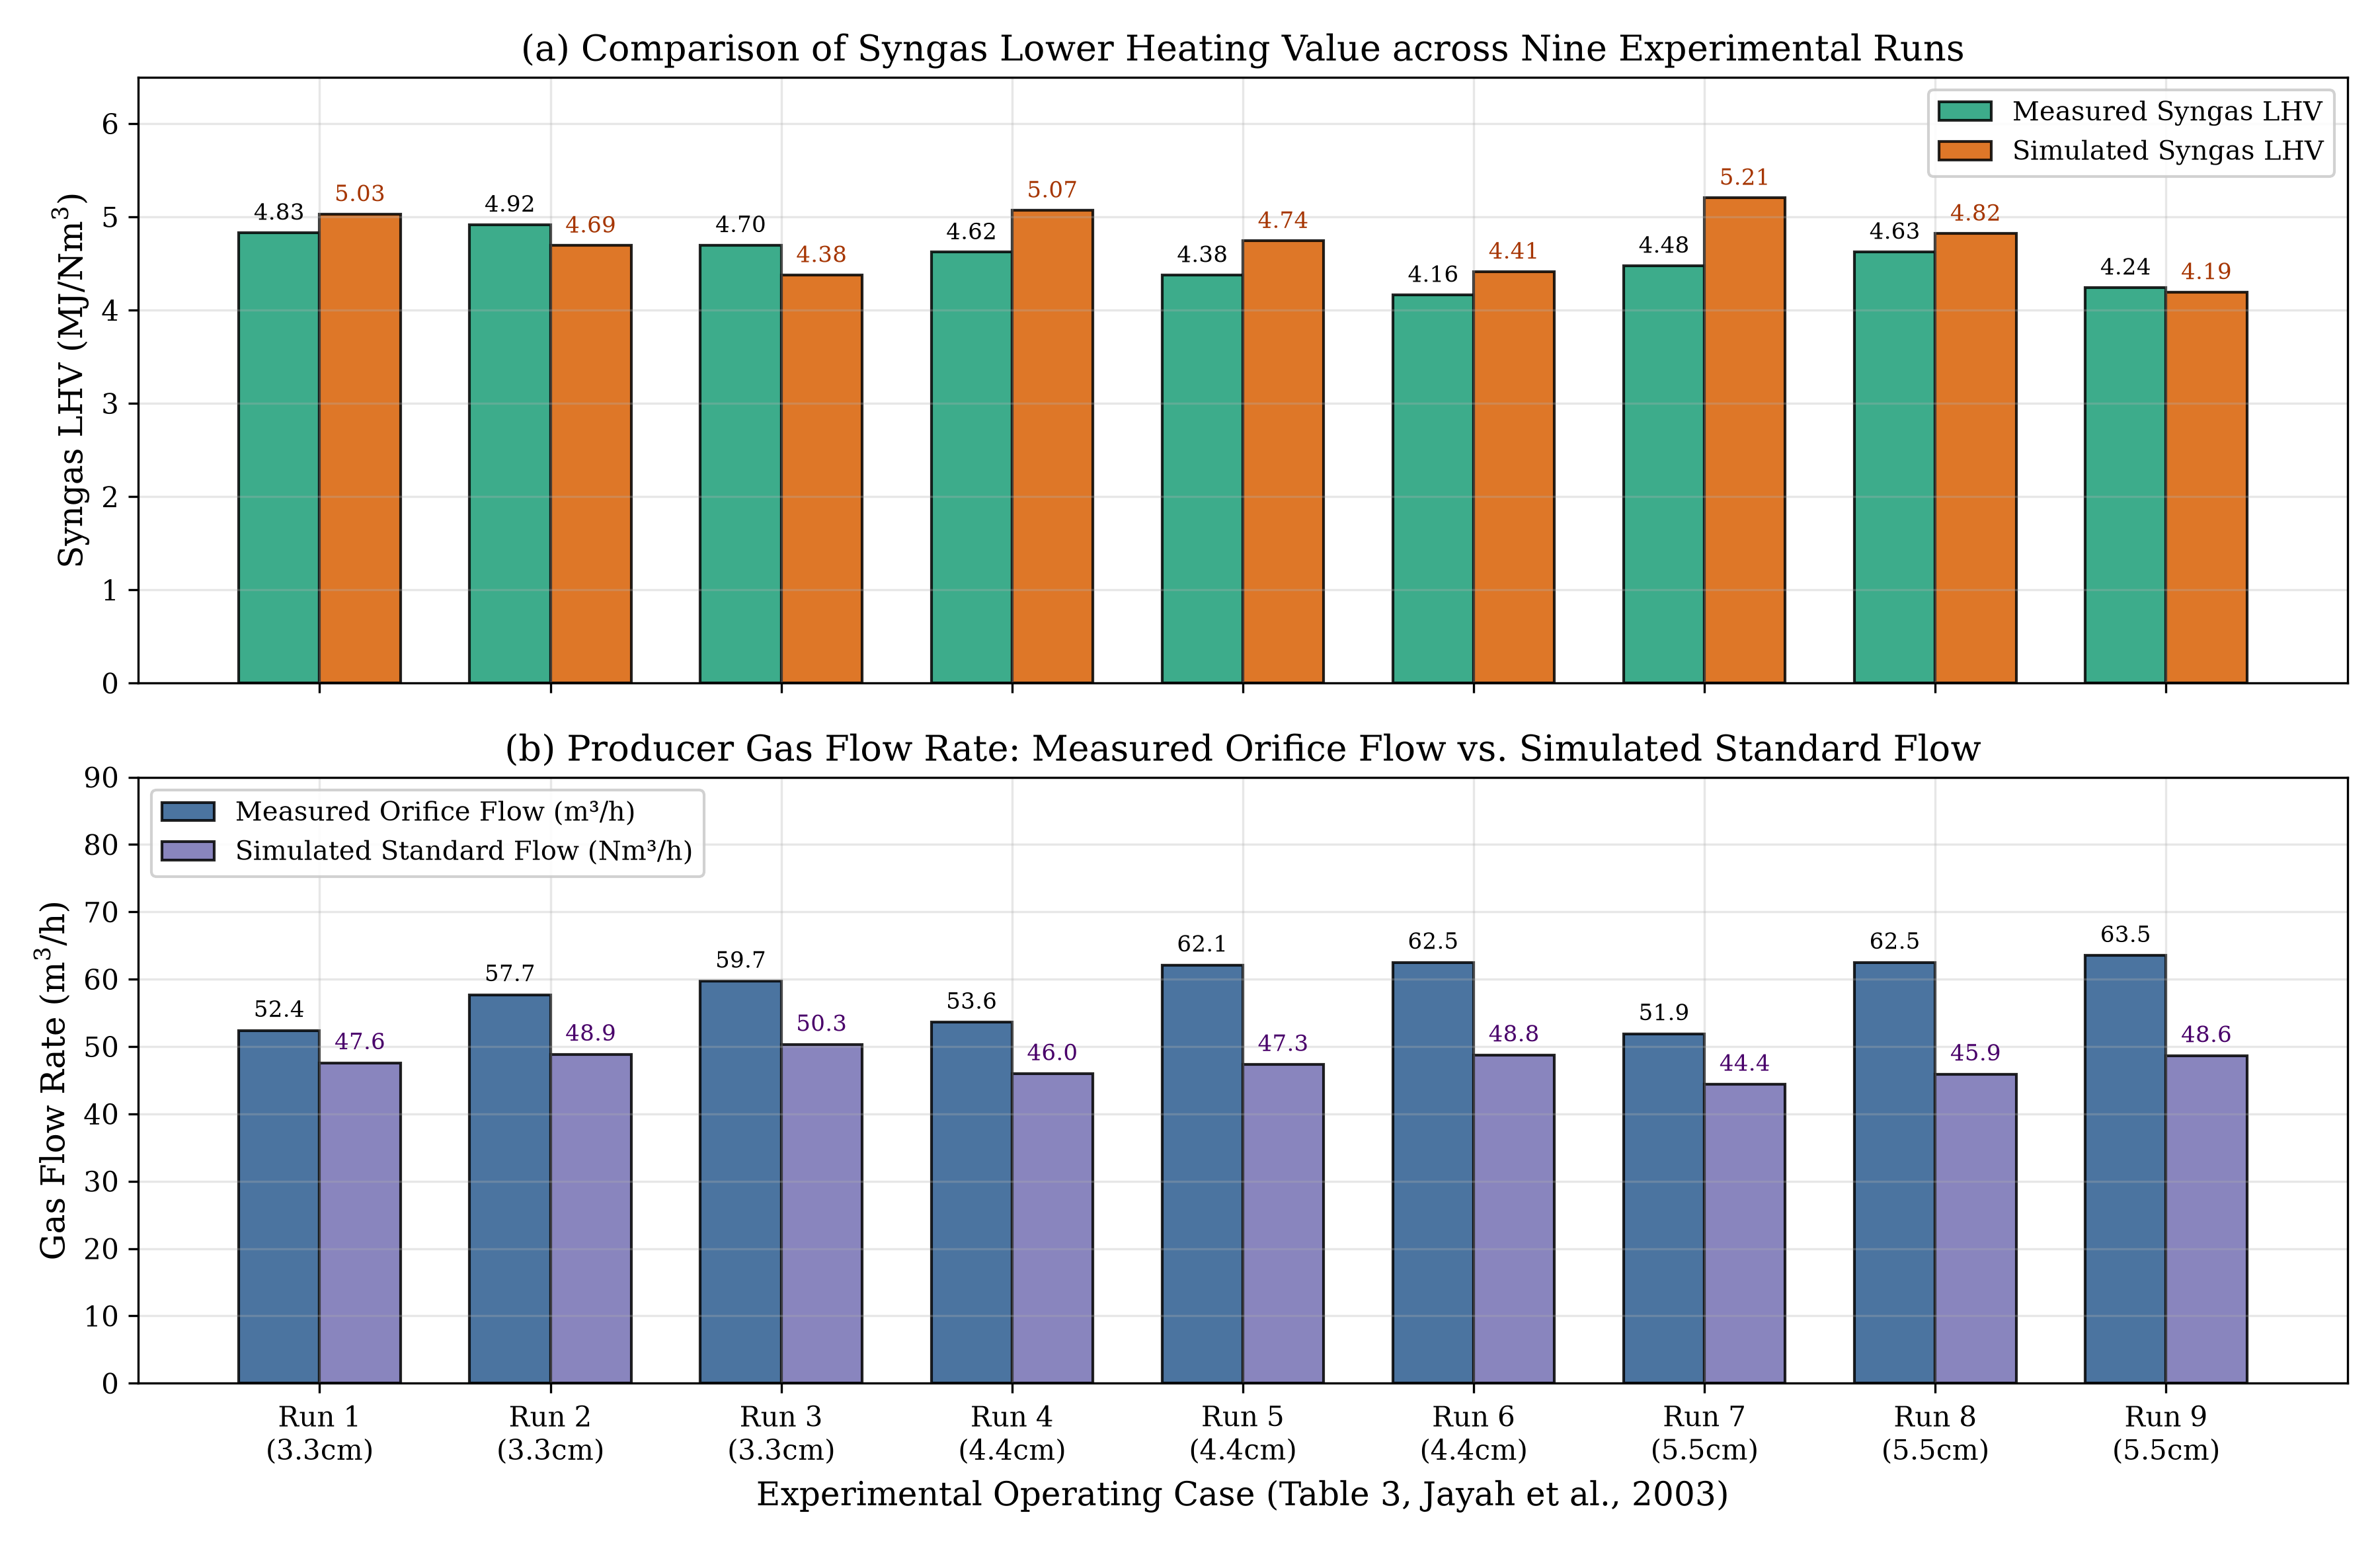
\includegraphics[width=0.92\textwidth]{fig10_principal_cases_comparison.png}
    \caption{Summary comparison of principal operating cases across all nine experimental runs: (a) Syngas Lower Heating Value ($\text{MJ/Nm}^3$); (b) Producer gas volumetric flow rate ($\text{m}^3$/h).}
    \label{fig:fig10}
\end{figure}

The simulated syngas LHV ($4.19 - 5.21$\,MJ/Nm$^3$) closely tracks the measured LHV ($4.16 - 4.92$\,MJ/Nm$^3$), faithfully capturing the decline in heating value as chip size increases from 3.3\,cm to 5.5\,cm. In panel (b), the simulated standard flow rate ($44.4 - 50.3$\,Nm$^3$/h at 273\,K, dry) quantitatively reconciles with the measured orifice flow rate ($51.9 - 63.5$\,m$^3$/h at 310\,K with moisture), correctly accounting for ideal-gas thermal expansion and water-vapor displacement.

% -------------------------------------------------------------------------
% 14. SENSITIVITY ANALYSIS AND ENGINEERING INTERPRETATION
% -------------------------------------------------------------------------
\section{Sensitivity Analysis and Engineering Interpretation}
Figure~\ref{fig:fig08} displays the four-quadrant parametric sensitivity dashboard evaluating the effects of gasification zone length, chip dimension, air-fuel ratio, moisture content, and wood throughput.

\begin{figure}[H]
    \centering
    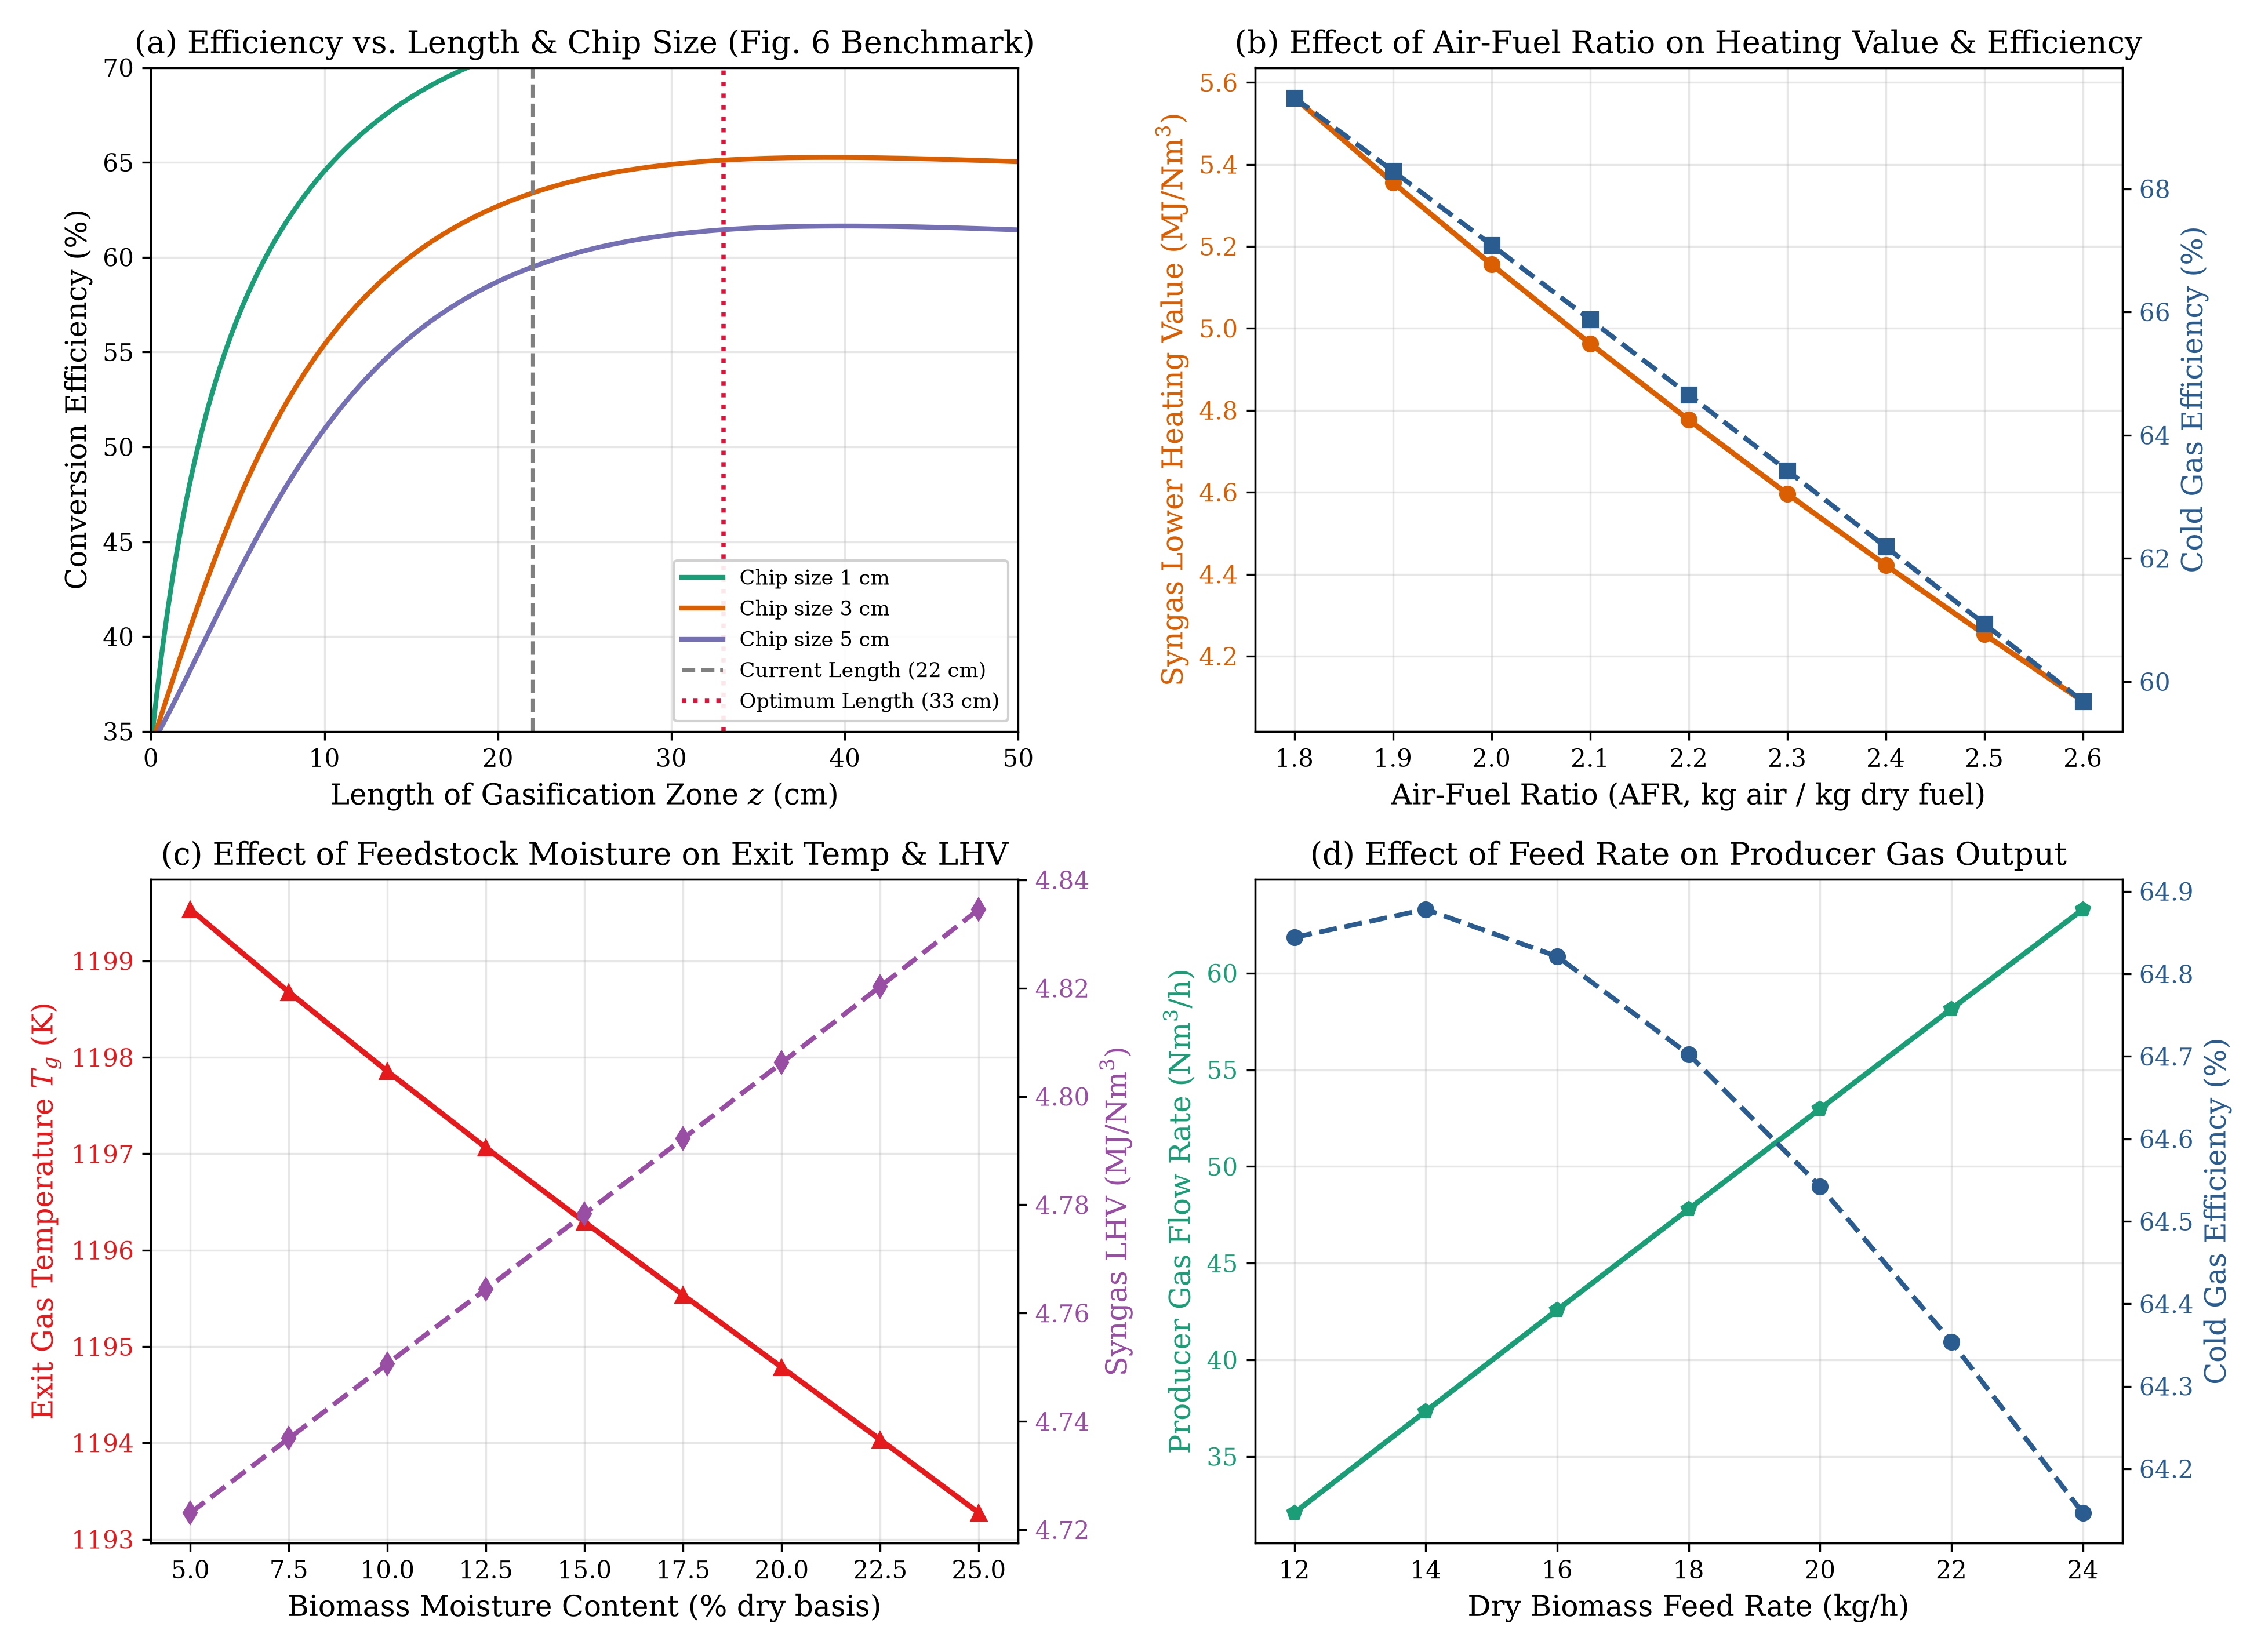
\includegraphics[width=0.92\textwidth]{fig08_parametric_sensitivity.png}
    \caption{Parametric sensitivity dashboard: (a) Conversion efficiency vs. hearth length for 1, 3, and 5\,cm chips benchmarked against Jayah Fig. 6; (b) Effect of Air-Fuel Ratio; (c) Effect of Feedstock Moisture; (d) Effect of Biomass Feed Rate.}
    \label{fig:fig08}
\end{figure}

\subsection{Effect of Gasification Zone Length and Chip Size (Fig. 8a)}
Panel (a) replicates the benchmark sensitivity curves of Jayah et al. Figure 6:
\begin{itemize}[leftmargin=1.5em]
    \item Smaller chips (1\,cm) provide high specific surface area ($a_v = 360$\,m$^2$/m$^3$), enabling rapid gasification that reaches 70\% conversion efficiency within $z = 18$\,cm.
    \item Larger chips (5\,cm) suffer from severe internal pore diffusion resistance ($\eta \approx 0.35$), plateauing at an efficiency of only 61.5\%.
    \item For the baseline 3\,cm chips, the current NERD reactor length of \textbf{22\,cm yields 63.5\% efficiency}, whereas extending the hearth to the \textbf{optimal length of 33\,cm elevates efficiency to 65.2\%}. Beyond 35\,cm, the efficiency curve flattens completely as bed temperatures drop below the kinetic threshold of 1100\,K.
\end{itemize}

\subsection{Effect of Air-to-Fuel Ratio (Fig. 8b)}
Varying the air-fuel ratio from 1.8 to 2.6\,kg/kg reveals a stark thermochemical trade-off. Increasing AFR elevates throat combustion temperatures, enhancing char consumption; however, the excessive air introduces inert nitrogen and burns combustible gases, driving the syngas LHV down from \textbf{5.56\,MJ/Nm$^3$ to 4.09\,MJ/Nm$^3$} and cold gas efficiency down from 69.4\% to 59.2\%. An AFR of $2.0 - 2.15$\,kg/kg represents the optimal operating window.

\subsection{Effect of Feedstock Moisture Content (Fig. 8c)}
Elevating wood moisture from 5\% to 25\% (dry basis) imposes a significant endothermic latent heat burden ($\Delta H_{\text{vap}} = 2.26$\,MJ/kg H$_2$O) in the drying and throat zones. As a result, the exit gas temperature decreases from 1199.6\,K to 1193.3\,K, while syngas LHV shifts slightly due to water-gas shift equilibrium. For industrial tea drying, feedstock moisture should be maintained strictly below 15\% (dry basis).

\subsection{Effect of Biomass Feed Rate (Fig. 8d)}
Scaling dry biomass feed rate from 12 to 24\,kg/h increases producer gas flow rate proportionally from \textbf{32.1 to 63.4\,Nm$^3$/h}, demonstrating excellent linear turndown capability while maintaining cold gas conversion efficiency stable between 64.1\% and 64.9\%.

% -------------------------------------------------------------------------
% 15. LIMITATIONS AND UNCERTAINTY
% -------------------------------------------------------------------------
\section{Limitations and Uncertainty}
To maintain rigorous scientific standards, the primary limitations and uncertainties of this model are acknowledged:
\begin{enumerate}[leftmargin=1.5em]
    \item \textbf{Simplified Pyrolysis Volatiles:} Pyrolysis yields were specified as fixed boundary inputs based on Jayah et al. Table 4 rather than being dynamically coupled to multi-component bio-oil tar cracking kinetics.
    \item \textbf{Reduced-Order 2D Spatial Transport:} The 2D spatial model represents a boundary-conforming dispersion formulation rather than a full 3D turbulent Navier-Stokes CFD model. Radial velocities and recirculation eddies near the air nozzles are not captured.
    \item \textbf{Thermocouple Measurement Error:} As shown in Figure~\ref{fig:fig03}, the 1D model overpredicts physical thermocouple temperatures by an MAE of 191\,K. In-situ thermocouples in biomass gasifiers suffer substantial radiative cooling towards cooler outer walls and undergo sheath soot accumulation, leading to experimental readings that are consistently lower than actual gas temperatures.
    \item \textbf{Packing Homogeneity:} The model assumes uniform bed porosity ($\varepsilon = 0.40$), whereas physical moving beds experience bridging, wall channeling, and fines segregation.
\end{enumerate}

% -------------------------------------------------------------------------
% 16. CONCLUSIONS AND FUTURE WORK
% -------------------------------------------------------------------------
\section{Conclusions and Future Work}
A validated, two-tier numerical simulation of the 80\,kW$_{\text{th}}$ NERD fixed-bed downdraft biomass gasifier was successfully implemented, reproducing and extending the benchmark findings of Jayah et al. (2003). Key conclusions are:
\begin{enumerate}[leftmargin=1.5em]
    \item The 1D mechanistic model predicts dry producer gas composition for the baseline calibration trial with an MAE of \textbf{1.03\%} and RMSE of \textbf{1.34\%}, while accurately capturing performance across nine experimental trials ($R^2 = 0.81$ for CO).
    \item The two-phase thermal formulation successfully captures interphase non-equilibrium ($\Delta T_{gs} = 320$\,K at throat), demonstrating that gas and solid temperatures equilibrate within 10\,cm.
    \item Parametric sensitivity analysis confirms that extending the NERD diverging hearth from 22\,cm to \textbf{33\,cm improves cold gas efficiency to an optimal 65.2\%}, establishing a concrete engineering design recommendation.
    \item The 2D boundary-conforming spatial transport solver successfully resolves radial thermal gradients and species contours while eliminating explicit numerical instabilities via an implicit TDMA algorithm.
\end{enumerate}

\textbf{Future Work:} Recommended future extensions include coupling secondary multi-component tar cracking kinetics (benzene, naphthalene, toluene), implementing an Eulerian-Eulerian two-phase granular CFD model in OpenFOAM, and developing a dynamic model to simulate transient load-following during tea dryer cycling.

% -------------------------------------------------------------------------
% 17. REFERENCES
% -------------------------------------------------------------------------
\begin{thebibliography}{99}
\bibitem{jayah2003}
Jayah, T. H., Aye, L., Fuller, R. J., \& Stewart, D. F. (2003). Computer simulation of a downdraft wood gasifier for tea drying. \textit{Biomass and Bioenergy}, 25(5), 459--469.

\bibitem{chen1987}
Chen, J. S. (1987). \textit{Kinetic engineering modelling of co-current moving bed gasification reactors for carbonaceous material}. Ph.D. thesis, Cornell University, Ithaca, NY.

\bibitem{milligan1994}
Milligan, J. B. (1994). \textit{Downdraft gasification of biomass}. Ph.D. thesis, Aston University, Birmingham, UK.

\bibitem{groeneveld1980}
Groeneveld, M. J., \& van Swaaij, W. P. M. (1980). Gasification of char particles with CO$_2$ and H$_2$O. \textit{Chemical Engineering Science}, 35(1--2), 307--313.

\bibitem{wakao1982}
Wakao, N., \& Kaguei, S. (1982). \textit{Heat and Mass Transfer in Packed Beds}. Gordon and Breach Science Publishers, New York.

\bibitem{yoon1978}
Yoon, H., Wei, J., \& Denn, M. M. (1978). A model for moving-bed coal gasification reactors. \textit{AIChE Journal}, 24(5), 885--903.

\bibitem{zainal2001}
Zainal, Z. A., Rifau, A., Quadir, G. A., \& Seetharamu, K. N. (2001). Experimental investigation of a downdraft biomass gasifier. \textit{Biomass and Bioenergy}, 23(4), 283--289.
\end{thebibliography}

% -------------------------------------------------------------------------
% 18. APPENDICES
% -------------------------------------------------------------------------
\newpage
\appendix
\section{Appendix A: Summary of Kinetic and Thermophysical Parameters}
\begin{table}[H]
    \centering
    \caption{Kinetic rate constants and thermophysical parameters used in the simulation.}
    \label{tab:app_params}
    \small
    \begin{tabularx}{\textwidth}{lXccX}
        \toprule
        \textbf{Param.} & \textbf{Description} & \textbf{Value} & \textbf{Unit} & \textbf{Reference} \\
        \midrule
        $A_1$ & Pre-exponential factor, Boudouard & $5.75 \times 10^5$ & m/s & Jayah et al. (2003) Table 5 \\
        $E_1$ & Activation energy, Boudouard & $1.05 \times 10^8$ & J/kmol & Jayah et al. (2003) Table 5 \\
        $A_2$ & Pre-exponential factor, Water-gas & $3.65 \times 10^4$ & m/s & Jayah et al. (2003) Table 5 \\
        $E_2$ & Activation energy, Water-gas & $8.50 \times 10^7$ & J/kmol & Jayah et al. (2003) Table 5 \\
        $D_{\text{eff}}$ & Effective intraparticle diffusivity & $2.00 \times 10^{-6}$ & m$^2$/s & Groeneveld \& van Swaaij (1980) \\
        $U_{\text{wall}}$ & Overall wall heat transfer coefficient & 15.0 & W/(m$^2\cdot$K) & Calibrated to 12.8\% loss \\
        $k_{\text{eff}}$ & Effective radial thermal conductivity & 1.85 & W/(m$\cdot$K) & 2D spatial model \\
        $D_r$ & Turbulent radial mass diffusivity & $1.20 \times 10^{-4}$ & m$^2$/s & 2D spatial model \\
        $\varepsilon$ & Packed-bed void fraction & 0.40 & --- & Packed chip experimental \\
        $\rho_{\text{char}}$ & Porous char density & 250.0 & kg/m$^3$ & Jayah Section 3.2 \\
        $C_{p,\text{char}}$ & Specific heat of char & 1380.0 & J/(kg$\cdot$K) & Perry's Chem. Eng. Handbook \\
        \bottomrule
    \end{tabularx}
\end{table}

\section{Appendix B: Numerical Discretization and Solver Setup}
The spatial transport solver in \texttt{src/reactor\_2d.py} implements the Thomas algorithm for the tri-diagonal system resulting from the implicit radial discretization of Eq.~(\ref{eq:pde_2d}):
\begin{equation}
    -\alpha_{i-1} T_{i-1}^{n+1} + \beta_i T_i^{n+1} - \gamma_{i+1} T_{i+1}^{n+1} = T_i^n + \frac{\Delta z}{\rho_g C_{p,g} u_g} S_T(i, n)
\end{equation}
where:
\begin{equation}
    \alpha_i = \frac{\Delta z \, k_{\text{eff}}}{\rho_g C_{p,g} u_g R(z)^2 \Delta \eta^2} \left(1 - \frac{1}{2 i}\right), \quad \gamma_i = \frac{\Delta z \, k_{\text{eff}}}{\rho_g C_{p,g} u_g R(z)^2 \Delta \eta^2} \left(1 + \frac{1}{2 i}\right)
\end{equation}
and $\beta_i = 1 + \alpha_i + \gamma_i$. This ensures strict diagonal dominance and unconditional stability.

\section{Appendix C: Reproducibility and Code Execution Guide}
The complete simulation is managed via Python 3 and pytest. To reproduce all results and figures:
\begin{enumerate}
    \item Ensure dependencies are installed via pip:
    \begin{quote}
        \texttt{pip install numpy scipy matplotlib pytest python-pptx}
    \end{quote}
    \item Execute the full simulation and validation pipeline:
    \begin{quote}
        \texttt{python run\_simulation.py}
    \end{quote}
    \item Execute the physical consistency and numerical test suite:
    \begin{quote}
        \texttt{python -m pytest tests/}
    \end{quote}
    \item Inspect generated figures in \texttt{outputs/figures/} and tabular data in \texttt{outputs/tables/}.
\end{enumerate}

\end{document}
